\ifx\allfiles\undefined
\documentclass[12pt, a4paper,oneside, UTF8]{ctexbook}
\usepackage[dvipsnames]{xcolor}
\usepackage{amsmath}   % 数学公式
\usepackage{amsthm}    % 定理环境
\usepackage{amssymb}   % 更多公式符号
\usepackage{graphicx}  % 插图
%\usepackage{mathrsfs}  % 数学字体
%\usepackage{newtxtext,newtxmath}
%\usepackage{arev}
\usepackage{kmath,kerkis}
\usepackage{newtxtext}
\usepackage{bbm}
\usepackage{enumitem}  % 列表
\usepackage{geometry}  % 页面调整
%\usepackage{unicode-math}
\usepackage[colorlinks,linkcolor=black]{hyperref}


\usepackage{ulem}	   % 用于更多的下划线格式,
					   % \uline{}下划线,\uuline{}双下划线,\uwave{}下划波浪线,\sout{}中间删除线,\xout{}斜删除线
					   % \dashuline{}下划虚线,\dotuline{}文字底部加点


\graphicspath{ {flg/},{../flg/}, {config/}, {../config/} }  % 配置图形文件检索目录
\linespread{1.5} % 行高

% 页码设置
\geometry{top=25.4mm,bottom=25.4mm,left=20mm,right=20mm,headheight=2.17cm,headsep=4mm,footskip=12mm}

% 设置列表环境的上下间距
\setenumerate[1]{itemsep=5pt,partopsep=0pt,parsep=\parskip,topsep=5pt}
\setitemize[1]{itemsep=5pt,partopsep=0pt,parsep=\parskip,topsep=5pt}
\setdescription{itemsep=5pt,partopsep=0pt,parsep=\parskip,topsep=5pt}

% 定理环境
% ########## 定理环境 start ####################################
\theoremstyle{definition}
\newtheorem{defn}{\indent 定义}[section]

\newtheorem{lemma}{\indent 引理}[section]    % 引理 定理 推论 准则 共用一个编号计数
\newtheorem{thm}[lemma]{\indent 定理}
\newtheorem{corollary}[lemma]{\indent 推论}
\newtheorem{criterion}[lemma]{\indent 准则}

\newtheorem{proposition}{\indent 命题}[section]
\newtheorem{example}{\indent \color{SeaGreen}{例}}[section] % 绿色文字的 例 ,不需要就去除\color{SeaGreen}{}
\newtheorem*{rmk}{\indent \color{red}{注}}

% 两种方式定义中文的 证明 和 解 的环境:
% 缺点:\qedhere 命令将会失效【技术有限,暂时无法解决】
\renewenvironment{proof}{\par\textbf{证明.}\;}{\qed\par}
\newenvironment{solution}{\par{\textbf{解.}}\;}{\qed\par}

% 缺点:\bf 是过时命令,可以用 textb f等替代,但编译会有关于字体的警告,不过不影响使用【技术有限,暂时无法解决】
%\renewcommand{\proofname}{\indent\bf 证明}
%\newenvironment{solution}{\begin{proof}[\indent\bf 解]}{\end{proof}}
% ######### 定理环境 end  #####################################

% ↓↓↓↓↓↓↓↓↓↓↓↓↓↓↓↓↓ 以下是自定义的命令  ↓↓↓↓↓↓↓↓↓↓↓↓↓↓↓↓

% 用于调整表格的高度  使用 \hline\xrowht{25pt}
\newcommand{\xrowht}[2][0]{\addstackgap[.5\dimexpr#2\relax]{\vphantom{#1}}}

% 表格环境内长内容换行
\newcommand{\tabincell}[2]{\begin{tabular}{@{}#1@{}}#2\end{tabular}}

% 使用\linespread{1.5} 之后 cases 环境的行高也会改变,重新定义一个 ca 环境可以自动控制 cases 环境行高
\newenvironment{ca}[1][1]{\linespread{#1} \selectfont \begin{cases}}{\end{cases}}
% 和上面一样
\newenvironment{vx}[1][1]{\linespread{#1} \selectfont \begin{vmatrix}}{\end{vmatrix}}

\def\d{\textup{d}} % 直立体 d 用于微分符号 dx
\def\R{\mathbb{R}} % 实数域
\def\N{\mathbb{N}} % 自然数域
\def\C{\mathbb{C}} % 复数域
\def\Z{\mathbb{Z}} % 整数环
\def\Q{\mathbb{Q}} % 有理数域
\newcommand{\bs}[1]{\boldsymbol{#1}}    % 加粗,常用于向量
\newcommand{\ora}[1]{\overrightarrow{#1}} % 向量

% 数学 平行 符号
\newcommand{\pll}{\kern 0.56em/\kern -0.8em /\kern 0.56em}

% 用于空行\myspace{1} 表示空一行 填 2 表示空两行  
\newcommand{\myspace}[1]{\par\vspace{#1\baselineskip}}

%s.t. 用\st就能打出s.t.
\DeclareMathOperator{\st}{s.t.}

%罗马数字 \rmnum{}是小写罗马数字, \Rmnum{}是大写罗马数字
\makeatletter
\newcommand{\rmnum}[1]{\romannumeral #1}
\newcommand{\Rmnum}[1]{\expandafter@slowromancap\romannumeral #1@}
\makeatother
\begin{document}
	% \title{{\Huge{\textbf{$Complex \,\, Analysis$\footnote{课堂教材:\textbf{《$Complex \,\, Analysis$》---  $Elias \,\, M. \,\, Stein$}}}}}}
\author{$-TW-$}
\date{\today}
\maketitle                   % 在单独的标题页上生成一个标题

\thispagestyle{empty}        % 前言页面不使用页码
\begin{center}
	\Huge\textbf{序}
\end{center}


\vspace*{3em}
\begin{center}
	\large{\textbf{天道几何,万品流形先自守;}}\\
	
	\large{\textbf{变分无限,孤心测度有同伦。}}
\end{center}

\vspace*{3em}
\begin{flushright}
	\begin{tabular}{c}
		\today \\ \small{\textbf{长夜伴浪破晓梦,梦晓破浪伴夜长}}
	\end{tabular}
\end{flushright}


\newpage                      % 新的一页
\pagestyle{plain}             % 设置页眉和页脚的排版方式(plain:页眉是空的,页脚只包含一个居中的页码)
\setcounter{page}{1}          % 重新定义页码从第一页开始
\pagenumbering{Roman}         % 使用大写的罗马数字作为页码
\tableofcontents              % 生成目录

\newpage                      % 以下是正文
\pagestyle{plain}
\setcounter{page}{1}          % 使用阿拉伯数字作为页码
\pagenumbering{arabic}
\setcounter{chapter}{-1}    % 设置 -1 可作为第零章绪论从第零章开始 
	\else
	\fi
	%  ############################ 正文部分

\chapter{课程要求}
	\begin{itemize}
		\item \textbf{任课教师}:林明华
		
		\item \textbf{辅导时间}:周一$9a.m. - 11a.m.$
		
		\item \textbf{办公室}:数学楼$210$
		
		\item \textbf{$Email$}:$mh.lin@xjtu.edu.cn$
		
		\item \textbf{总评成绩组成}:阅读报告及汇报$20\%$ + 期末考试$80\%$
	\end{itemize}

\chapter{$Week \,\, 1$}
\section{复数的引入}
\paragraph{引入}
	\begin{center}
		下面从代数结构($Group , \,\, Ring , \,\, Field$)的角度引入复数的概念.
	\end{center}
	$Consider \,\, the \,\, set \,\, \R^2 . \,\, Define \,\, two \,\, operations . \,\, \forall (a , b) , (c , d) \in \R^2 , $
	\begin{align}
		(a , b) + (c , d) &\coloneqq (a + c , b + d)\\
		(a , b) \cdot (c , d) &\coloneqq (ac - bd , bc + ad)
	\end{align}
	$"\cdot" \,\, is \,\, commutative.$\\
	$"+" , \,\, "\cdot" \,\, satisfy \,\, associative \,\, and \,\, distributive \,\, laws.$
	\begin{align}
		(0 , 0) &: The \,\, additive \,\, identity \\
		(1 , 0) &: The \,\, multiplicative \,\, identity
	\end{align}
	$\Rightarrow (\R^2 , \,\, + , \,\, \cdot) \,\, is \,\, a \,\, communicative \,\, ring.$
	
	\vspace*{2em}
	$\forall (a , b) \in \R^2 , \,\, (a , b) \neq (0 , 0) , \,\, if$
	\begin{align}
		&(a , b) \cdot (x , y) = (1 , 0) \\
		&\Rightarrow x = \frac{a}{a^2 + b^2} , \,\, y = \frac{-b}{a^2 + b^2}
	\end{align}
	$Therefore , \,\, (\R^2 , \,\, + , \,\, \cdot) \,\, is \,\, a \,\, field , \,\, renoted \,\, as \,\, \C.$
	
\vspace*{2em}
\paragraph{复数的乘法}
	在上述对$\C$ 的定义中,唯一非平凡的点便是乘法运算$"\cdot"$ 的定义.
\begin{center}
	下面我们从代数的方法,从另一个角度理解复数的乘法.
\end{center}
	$We \,\, may \,\, ask \,\, a \,\, question \,\, : \,\, \uwave{Can \,\, we \,\, define \,\, a \,\, "\cdot" \,\, and  \,\, let \,\, (\R^3 , \,\, + , \,\, \cdot) \,\, be \,\, a \,\, field?}$\\
	$However , \,\, the \,\, answer \,\, is \,\, certainly \,\, not !$
	
	\vspace*{2em}
		$Consider \,\, M_2 = 
		\left\{ 
		\begin{pmatrix}
			a \,\, &-b\\
			b \,\, &a
		\end{pmatrix} \,\, \Bigg| \,\, a , b \in \R
		\right\}
		\,\, equipped \,\, with \,\, the \,\, usual \,\, matrix \,\, addition \,\, and \,\, multiplication.$\\
		
	$Define \,\, a \,\, map \,\, \sigma.$
	\begin{align}
		\sigma : \R^2 &\longrightarrow M_2 \\
		(a , b) &\longmapsto 
		\begin{pmatrix}
			a \,\, &-b\\
			b \,\, &a
		\end{pmatrix}
	\end{align}
	$Then , \,\, \sigma \,\, is \,\, bijective.$
	\begin{align}
		\sigma(a , b) \cdot \sigma(c , d) = 
		\begin{pmatrix}
			a \,\, &-b\\
			b \,\, &a
		\end{pmatrix} 
		\begin{pmatrix}
			c \,\, &-d\\
			d \,\, &c
		\end{pmatrix}
		= 
		\begin{pmatrix}
			ac - bd \,\, &-(bc + ad)\\
			bc + ad \,\, &ac - bd
		\end{pmatrix}
		= 
		\sigma((a , b) \cdot (c , d))
	\end{align}
	$\Rightarrow \sigma \,\, is \,\, an \,\, isomorphism(\text{同构映射}).$ \\
	于是复数乘法可视作复平面上带伸缩的旋转.	
	
\newpage
\section{复数的基本性质}
\paragraph{$Some \,\, Facts$}
	\begin{align}
		\left| Rez \right| \leq \left| z \right| &, \,\, \left| Imz \right| \leq \left| z \right| \\
		Rez = \frac{z + \bar{z}}{2} &, \,\, Imz = \frac{z - \bar{z}}{2i}
	\end{align}

\vspace*{2em}
\paragraph{性质}
	下面给出一些命题.
	\begin{enumerate}
		\item 三角不等式.
		\begin{proposition}[$Triangle \,\, Inequality$]
			$Let \,\, z , w \in \C . \,\, Then$
			\begin{align}
				\left| z + w \right| \leq \left| z \right| + \left| w \right|
			\end{align}
			
			\begin{proof}
				$Let \,\, z = a + bi , \,\, w = c + di . \,\, Then$
				\begin{align}
					&\Leftrightarrow \sqrt{(a + c)^2 + (b + d)^2} \leq \sqrt{a^2 + b^2} + \sqrt{c^2 + d^2} \\
					&\Leftrightarrow ac + bd \leq \sqrt{(a^2 + b^2)(c^2 + d^2)} = \sqrt{(ac)^2 + (bd)^2 + a^2 d^2 + b^2 c^2}
				\end{align}
			\end{proof}
		\end{proposition}
	
		\begin{corollary}
			$If \,\, z , w \in \C , \,\, then$
			\begin{align}
				\left| \left| z \right| - \left| w \right| \right| \leq \left| z - w \right|
			\end{align}
		
			\begin{proof}
				\begin{align}
					\left| z \right| &= \left| z - w + w \right| \leq \left| z - w \right| + \left| w \right| \\
					\left| w \right| &= \left| z - w - z \right| \leq \left| z - w \right| + \left| z \right| \\
					\Rightarrow \left| z - w \right| 
					&\geq max\left\{ \left| z \right| - \left| w \right| , \,\, \left| w \right| - \left| z \right| \right\} 
					= \left| \left| z \right| - \left| w \right| \right|
				\end{align}
			\end{proof}
		\end{corollary}
	
		\item $Cauchy - Schwarz$ 不等式.
		\begin{proposition}[$Cauchy - Schwarz$]
			$Let \,\, z_1 , \cdots , z_n , w_1 , \cdots , w_n \in\C . \,\, Then$
			\begin{align}
				\left| \sum_{k = 1}^{n}{z_k w_k} \right|^2 \leq 
				\left( \sum_{k = 1}^{n}{\left| z_k \right|^2} \right)
				\left( \sum_{k = 1}^{n}{\left| w_k \right|^2} \right)
			\end{align}
		
			\begin{proof}
				$\forall \lambda \in \R , \,\, \vartheta \in \R ,$
				\begin{align}
					0 \leq 
					\sum_{k = 1}^{n}{\left| z_k - \lambda e^{i\vartheta} \overline{w_k} \right|^2} 
					&= \sum_{k = 1}^{n}
					{(z_k - \lambda e^{i\vartheta} \overline{w_k}) (\overline{z_k} - \lambda e^{-i\vartheta} w_k)}\\
					&= \sum_{k = 1}^{n}{\left| z_k \right|^2} - 2\left( Re \,\, e^{-i\vartheta} 
					\sum_{k = 1}^{n}{z_k w_k} \right) \lambda + \lambda^2 \sum_{k = 1}^{n}{\left| w_k \right|^2}\\
					&= a \lambda^2 - 2b \lambda + c \\
					&\Rightarrow b^2 \leq ac
				\end{align}
				$Then$
				\begin{align}
					\left( Re \,\, e^{-i\vartheta} \sum_{k = 1}^{n}{z_k w_k} \right)^2 \leq 
					\left( \sum_{k = 1}^{n}{\left| z_k \right|^2} \right)
					\left( \sum_{k = 1}^{n}{\left| w_k \right|^2} \right) 
				\end{align}
				$Suppose \,\, z = \sum_{k = 1}^{n}{z_k w_k} = \left| z \right| e^{i \varphi} \in \C , \,\, let \,\, \vartheta = \varphi . \,\, Then$
				\begin{align}
					Re \,\, e^{-i\vartheta} \sum_{k = 1}^{n}{z_k w_k} &= \left| \sum_{k = 1}^{n}{z_k w_k} \right| \\
					\left| \sum_{k = 1}^{n}{z_k w_k} \right|^2 &\leq 
					\left( \sum_{k = 1}^{n}{\left| z_k \right|^2} \right)
					\left( \sum_{k = 1}^{n}{\left| w_k \right|^2} \right)
				\end{align}
			\end{proof}
		\end{proposition}
	\end{enumerate}

\newpage
\section{课堂例题$2024-02-26$}
	\begin{enumerate}
		\item $Let \,\, z_1 , z_2 \in \C , \,\, \left| z_1 \right| \leq 1 , \,\, \left| z_2 \right| \leq 1 . \,\, If \,\, \left| z_1 - z_2 \right| \geq 1 , \,\, show \,\, that$
		\begin{align}
			\left| z_1 + z_2 \right| \leq \sqrt{3}
		\end{align}
	
	\vspace*{2em}
	\begin{proof}
		(平行四边形对角线的平方和等于四边的平方和.)
		\begin{align}
			\left| z_1 - z_2 \right|^2 
			&= (z_1 - z_2)(\overline{z_1} - \overline{z_2})
			= \left| z_1 \right|^2 + \left| z_2 \right|^2 - z_1 \overline{z_2} - \overline{z_1} z_2\\
			\left| z_1 + z_2 \right|^2 
			&= (z_1 + z_2)(\overline{z_1} + \overline{z_2})
			= \left| z_1 \right|^2 + \left| z_2 \right|^2 + z_1 \overline{z_2} + \overline{z_1} z_2
		\end{align}
		$\Rightarrow$
		\begin{align}
			\left| z_1 - z_2 \right|^2 + \left| z_1 + z_2 \right|^2 
			&= 2(\left| z_1 \right|^2 + \left| z_2 \right|^2) \\
			\left| z_1 + z_2 \right|^2 
			&= 2(\left| z_1 \right|^2 + \left| z_2 \right|^2) - \left| z_1 - z_2 \right|^2 
			\leq 3
		\end{align}
	\end{proof}

	\vspace*{3em}

	\item $Let \,\, z_1 , \cdots , z_n \in \C , \,\, and \,\, let \,\, e_0 , e_1 , \cdots , e_{n + 1} \in \C \,\, be \,\, the \,\, coefficients \,\, of \,\, (z + 1) \overset{n}{\underset{k = 1}{\prod}}{(z + z_k)} , $\\
	$i.e.$
	\begin{align}
		(z + 1) \prod_{k = 1}^{n}{(z + z_k)} = \sum_{k = 0}^{n + 1}{e_k z^{n + 1 - k}}
	\end{align}
	$Show \,\, that \,\, \overset{n + 1}{\underset{k = 0}{\sum}}{(k + 1) e_k z^{n + 1 - k}} = 0 \,\, has \,\, a \,\, root \,\, of \,\, modulus \,\, \geq 1 .$
	
	\vspace*{2em}
	$Specifically , \,\, try \,\, to \,\, show \,\, n = 1 \,\, case . $\\
	$\Leftrightarrow (Let \,\, c \in \C , \,\, show \,\, z^2 + 2(1 + c)z + 3c = 0 \,\, has \,\, a \,\, root \,\, of \,\, modulus \,\, \geq 1 .)$
	
	\vspace*{2em}
	\begin{proof}
		下面对方程$z^2 + 2(1 + c)z + 3c = 0$ 的根的情况进行分类(事实上同时对$c \in \C$ 的取值进行了分类).
		\begin{enumerate}
			\item[(1)]若方程存在实根$z_0 \in \R$,下面可以证明,事实上$(1) \Leftrightarrow c \in \R$.
			\begin{align}
				&z_{0}^2 + 2(1 + c)z_{0} + 3c = 0 \\
				&\Rightarrow (2z_{0} + 3)c = -z_{0}^2 - 2z_0 \\
				&\Rightarrow c = \frac{-z_{0}^2 - 2z_0}{2z_{0} + 3} \in \R \,\, 
				\text{或} \,\, z_0 = \frac{3}{2}(\textbf{此时$-z_{0}^2 - 2z_0 \neq 0$ 矛盾})
			\end{align}
			于是$c \in \R , \,\, z^2 + 2(1 + c)z + 3c = 0$ 为实系数一元二次方程.
			\begin{align}
				\Delta &= 4(1 + c)^2 - 12c = 4(c^2 - c + 1) > 0 , \,\, \forall c \in \R \\
				z &= - 1 - c \pm \sqrt{c^2 - c + 1} \in \R
			\end{align}
			下面再对实数$c \in \R$ 的范围分类讨论.
			\begin{enumerate}
				\item[\rmnum{1}).]$c \geq 0$,则其中一根$z = - 1 - c - \sqrt{c^2 - c + 1} < - 1 , \,\, \left| z \right| > 1$.
				
				\item[\rmnum{2}).]$c < 0$,考虑其中一根
				\begin{align}
					z &= - 1 - c - \sqrt{c^2 - c + 1} \\
					&= - 1 - (\sqrt{c^2 - c + 1} + c)
				\end{align}
				由于$c < 0$,因此$1 - c > 0$.
				\begin{align}
					\sqrt{c^2 - c + 1} = \sqrt{c^2 + (1 - c)} &> \sqrt{c^2} = \left| c \right| \\
					\sqrt{c^2 - c + 1} + c &> 0 \\
					z = - 1 - (\sqrt{c^2 - c + 1} + c) &< - 1 \\
					\left| z \right| &> 1
				\end{align}
			\end{enumerate}
			于是对于$\forall c \in \R$,都有$\left| z \right| > 1$.从而得证.\\
			事实上,根据上述证明过程可知,若$c \in \R$,则原方程必有实根,且两根均为实根,从而
			\begin{align}
				(1) : \text{方程存在实根} \Leftrightarrow c \in \R \Leftrightarrow \text{两根均为实根}
			\end{align}
		
			\vspace*{2em}
			\item[(2)]若方程无实根,即$c \in \C$
		\end{enumerate}
	\end{proof}
	\end{enumerate}

\newpage
\section{复数域$\C$ 上的拓扑概念$\&$ 性质}
	$Let \,\, \alpha \in \C , \,\, open \,\, disc \,\, of \,\, radius \,\, r \,\, centered \,\, at \,\, \alpha$
	\begin{align}
		D_r (\alpha) &\coloneqq \{ z \in \C \mid \left| z - \alpha \right| < r \} \\
		D_{r}^{*} (\alpha) &\coloneqq \{ z \in \C \mid 0 < \left| z - \alpha \right| < r \}
	\end{align}
	$closed \,\, disc \,\, of \,\, radius \,\, r \,\, centered \,\, at \,\, \alpha$
	\begin{align}
		\overline{D}_r (\alpha) &\coloneqq \{ z \in \C \mid \left| z - \alpha \right| \leq r \}
	\end{align}
	$unit \,\, disc:$
	\begin{align}
		\mathbb{D} \coloneqq D_1 (0)
	\end{align}

\vspace*{2em}
	$Let \,\, \Omega \subseteq \C$
	\begin{defn}
		$\alpha \in \Omega \,\, is \,\, an \,\, \underline{interior \,\, point \,\, of \,\, \Omega} \,\, if \,\, \exists r > 0 , \,\, \st D_{r}(\alpha) \subseteq \Omega.$
		
		\begin{rmk}
			$The \,\, set \,\, of \,\, all \,\, interior \,\, points \,\, of \,\, \Omega \,\, is \,\, called \,\, \underline{the \,\, interior \,\, of \,\, \Omega} , \,\, denoted \,\, by \,\, Int(\Omega).$
		\end{rmk}
	\end{defn}

\vspace*{2em}
	
	\begin{defn}
		$\Omega \,\, is \,\, open \,\, if \,\, \Omega = Int(\Omega).$
		\begin{rmk}
			$\C \,\, is \,\, open . \,\, \varnothing \,\, is \,\, open . \,\,(by \,\, convention)$
		\end{rmk}
	\end{defn}

\vspace*{2em}

	\begin{defn}
		$\Omega \,\, is \,\, closed \,\, if \,\, \Omega^c \coloneqq \C \backslash \Omega \,\, is \,\, open.$
	\end{defn}

\vspace*{2em}

	\begin{thm}
		$Every \,\, Cauchy \,\, sequence \,\, in \,\, \C \,\, has \,\, a \,\, limit \,\, in \,\, \C . \,\, That \,\, is , \,\, \C \,\, is \,\, Complete.$
	\end{thm}




\newpage
\section{课堂例题$2024-03-01$}
	\begin{enumerate}
		\item 
		\begin{align}
			\lim_{n \to +\infty}{z_n} = w \Leftrightarrow \lim_{n \to +\infty}{Re z_n} = Re w , \,\, \lim_{n \to +\infty}{Im z_n} = Im w
		\end{align}
		
		\vspace*{2em}
		\begin{proof}
			\begin{enumerate}
				\item[$\Rightarrow$]:$\left| Re z_n - Re w \right| = \left| Re (z_n - w) \right| \leq \left| z_n - w \right|$
				
				\item[$\Leftarrow$]:$\left| z_n - w \right| 
				\leq \left| Re (z_n - w) \right| + \left| Im (z_n - w) \right|
				= \left| Re z_n - Re w \right| + \left| Im z_n - Im w \right|$
			\end{enumerate}
		\end{proof}
	
		\vspace*{2em}
		\item $z \,\, is \,\, a \,\, limit \,\, point \,\, of \,\, \Omega \,\,\Leftrightarrow \,\, z \,\, is \,\, an \,\, accumulation \,\, point \,\, of \,\, \Omega$
		
		\vspace*{2em}
		\begin{proof}
			\begin{enumerate}
				\item[$\Rightarrow$]:$\forall r > 0 , \,\, \exists N_r , \,\, \st n > N , \,\, where \,\, z_n \in \Omega , \,\, z_n \neq z$.\\
				$z_n \in D_{r}^{*}(z) , \,\, z_n \in \Omega , \,\, \forall n > N_r$.\\
				$Hence \,\, z_n \in D_{r}^{*}(z) \cap \Omega \neq \varnothing , \,\, \forall r > 0 , \,\, n > N_r , \,\, i.e. \,\,$\\
				$z \,\, is \,\, an \,\, accumulation \,\, point \,\, of \,\, \Omega$
				
				\item[$\Leftarrow$]:$Take \,\, a \,\, point \,\, z_n \,\, from \,\, D_{\frac{1}{n}}^{*}(z) \cap \Omega \,\, which \,\, is \,\, not \,\, empty.$\\
				$Then \,\, \{ z_n \} \,\, is \,\, a \,\, Cauchy \,\, sequence \,\, which \,\, converges \,\, to \,\, z.$\\
				$Hence \,\, z \,\, is \,\, a \,\, limit \,\, point \,\, of \,\, \Omega.$
			\end{enumerate}
		\end{proof}
		\begin{rmk}
			$A \,\, limit \,\, point \,\, of \,\, \Omega \,\, may \,\, not \,\, belong \,\, to \,\, \Omega.$
		\end{rmk}
	
		\vspace{2em}
		
		\item 课本第一章练习$T3 , T5 , T7$.
	\end{enumerate}

\chapter{$Week \,\, 2 \,\, -- \,\, Functions \,\, on \,\, \C$}
\section{连续函数和极值}
	\begin{defn}\label{def 2.1.1}
		$Let \,\, \Omega \subseteq \C \,\, be \,\, open. \,\, We \,\, say \,\, f : \Omega \longrightarrow \C \,\, is \,\, continuous \,\, at \,\, z_0 \in \Omega \,\, $\\
		$if \,\, \forall \epsilon > 0 , \exists \delta > 0 , \st$
		\begin{align}
			whenever \,\, \left| z - z_0 \right| < \delta , \,\, z \in \Omega , \,\, then \,\, \left| f(z) - f(z_0) \right| < \epsilon
		\end{align}
		$To \,\, say \,\, it \,\, another \,\, way , \,\, \forall \epsilon > 0 , \exists \delta > 0 , \st \,\, f(D_{\delta}(z_0) \cap \Omega) \subseteq D_{\epsilon}(f(z_0))$
		
		\begin{rmk}
			$We \,\, say \,\, f \,\, is \,\, continuous \,\, on \,\, \Omega \,\, if \,\, f \,\, is \,\, continuous \,\, at \,\, every \,\, point \,\, of \,\, \Omega.$
		\end{rmk}
	\end{defn}
	
	\vspace*{2em}
	$Here \,\, are \,\, some \,\, facts.$
	\begin{enumerate}
		\item[$Fact \,\, 1.$] $If \,\, f \,\, is \,\, continuous \,\, on \,\, \Omega , \,\, then \,\, so \,\, are \,\, \overline{f} , \,\, \left| f \right| , \,\, \frac{1}{f} \,\, (if \,\, f(z) \neq 0 \,\, for \,\, all \,\, z \in \Omega).$
		\begin{proof}
			$For \,\, \left| f \right| , \,\, use \,\, \left| \left| f(z) \right| - \left| f(z_0) \right| \right| \leq \left| f(z) - f(z_0) \right|$
		\end{proof}
	
		\item[$Fact \,\, 2.$]$f \,\, is \,\, continuous \,\, iff \,\, Ref \,\, and \,\, Imf \,\, are \,\, continuous.$
	\end{enumerate}

	\vspace*{2em}
	\begin{proposition}\label{prop 2.1.1}
		$Let \,\, \Omega \subseteq \C \,\, and \,\, let \,\, f \,\, be \,\, continuous \,\, on \,\, \Omega . \,\, Then$
		\begin{enumerate}
			\item[(1)]$For \,\, every \,\, open \,\, set \,\, S \subseteq \C , \,\, f^{-1}(S) = \{ z \in \Omega \mid f(z) \in S \} \,\, is \,\, open.$
			
			\item[(2)]$For \,\, every \,\, compact \,\, set \,\, K \subseteq \C , \,\, f(K) \,\, is \,\, compact.$
		\end{enumerate}
	
		\vspace*{2em}
		\begin{proof}
			\begin{enumerate}
				\item[(1)]$If \,\, f^{-1}(S) = \varnothing , \,\, true.$\\
				$Assume \,\, f^{-1}(S) \neq \varnothing \,\, and \,\, let \,\, z_0 \in f^{-1}(S) . \,\, Write \,\, w_0 = f(z_0) \in S.$\\
				$Since \,\, S \,\, is \,\, open , \,\, \exists \epsilon > 0 , \st \,\, D_{\epsilon}(w_0) \subseteq S$\\
				$Since \,\, f \,\, is \,\, continuous , \,\, taking \,\, \epsilon \,\, in \,\, the \,\, definition , \,\, we \,\, get \,\, a \,\, \delta > 0 , \st$
				\begin{align}
					D_{\delta}(z_0) \subseteq \Omega \,\, and \,\, f(D_{\delta}(z_0)) \subseteq D_{\epsilon}(f(z_0)) = D_{\epsilon}(w_0) \subseteq S
				\end{align}
				$Thus \,\, D_{\delta}(z_0) \subseteq f^{-1}(S) , \,\, and \,\, so \,\, f^{-1}(S) \,\, is \,\, open.$
				
				\vspace*{2em}
				
				\item[(2)]$Let \,\, \{ \Omega_j \}_{j \in J} \,\, be \,\, an \,\, open \,\, cover \,\, of \,\, f(K) , \,\, i.e.$
				\begin{align}
					f(K) \subseteq \bigcup_{j \in J}{\Omega_j}
				\end{align}
				$Then$
				\begin{align}
					K \subseteq f^{-1}(\bigcup_{j \in J}{\Omega_j}) = \bigcup_{j \in J}{f^{-1}(\Omega_j)}
				\end{align}
				$By \,\, (1) , \,\, f^{-1}(\Omega_j) \,\, is \,\, open \,\, for \,\, all \,\, j \in J. \,\, Thus \,\, \{ f^{-1}(\Omega_j) \}_{j \in J} \,\, is \,\, an \,\, open \,\, cover \,\, of \,\, K.$\\
				$Since \,\, K \,\, is \,\, compact , \,\, \exists j_1 , \cdots , j_n \in J , \st $
				\begin{align}
					&k \subseteq \bigcup_{k = 1}^{n}{f^{-1}(\Omega_{j_k})} = f^{-1}(\bigcup_{k = 1}^{n}{\Omega_{j_k}}) \\
					&\Rightarrow f(K) \subseteq \bigcup_{k = 1}^{n}{\Omega_{j_k}}
				\end{align}
			\end{enumerate}
		\end{proof}
	\end{proposition}

	\vspace*{2em}
	$We \,\, say \,\, that \,\, f \,\, contains \,\, a \,\, maximum \,\, at \,\, z_0 \in \Omega \,\, if $
	\begin{align}
		\left| f(z) \right| \leq \left| f(z_0) \right| , \,\, \forall z \in \Omega
	\end{align}

	\begin{proposition}\label{prop 2.1.2}
		$A \,\, continuous \,\, function \,\, on \,\, a \,\, compact \,\, set \,\, \Omega \,\, is \,\, bounded \,\, and \,\, attains \,\, a \,\, maximum $\\ 
		$and \,\, a \,\, minimum \,\, on \,\, \Omega.$
		
		\vspace*{2em}
		\begin{proof}
			$use \,\, \left| f \right|^2 = (Ref)^2 + (Imf)^2$.
		\end{proof}
	\end{proposition}

\newpage
\section{复变函数的极限,全纯函数}
	\begin{defn}\label{def 2.2.1}
		$Assume \,\, \Omega \subseteq \C , \,\, \Omega \neq \varnothing \,\, and \,\, \alpha \in Acc(\Omega) , \,\, f : \Omega \longrightarrow \C , \,\, \underset{z \to \alpha , \, z \in \Omega}{\lim}{f(z)} = w \,\, means$
		\begin{align}
			\forall \epsilon > 0 , \exists \delta > 0 , \st \,\, 0 < \left| z - z_0 \right| < \delta \,\, \Rightarrow \,\, \left| f(z) - w \right| < \epsilon
		\end{align}
	
		\begin{rmk}
			容易证明若极限存在,则极限唯一.
		\end{rmk}
	\end{defn}

	\vspace*{2em}
	\begin{defn}\label{def 2.2.2}
		$Let \,\, \Omega \subseteq \C \,\, be \,\, open , \,\, f : \Omega \longrightarrow \C . \,\, We \,\, say \,\, f(z) \,\, is \,\, \underline{\textbf{$Complex \,\, differentiable \,\, at \,\, z_0 \in \Omega$}}$\\
		$if \,\, \underset{h \to 0}{\lim}{\frac{f(z_0 + h) - f(z_0)}{h}} \,\, exists. \,\, If \,\, f \,\, is \,\, complex \,\, differentiable at \,\, z_0 , \,\, we \,\, denote \,\, the \,\, limit \,\, of \,\, the \,\, quotient $\\ 
		$by \,\, f^{'}(z_0) . \,\, i.e.$
		\begin{align}
			f^{'}(z_0) = \lim_{h \to 0}{\frac{f(z_0 + h) - f(z_0)}{h}}
		\end{align}
		$f^{'}(z_0) \,\, is \,\, called \,\, \underline{\textbf{$the \,\, derivative \,\, of \,\, f \,\, at \,\, z_0$}}$.
		
		\begin{rmk}
			$If \,\, f \,\, is \,\, complex \,\, differentiable \,\, at \,\, every \,\, point \,\, of \,\, \Omega , \,\, then \,\, we \,\, say \,\, f \,\, is \,\, \underline{\textbf{$holomorphic$}} \,\, on \,\,  \Omega.$
		\end{rmk}
	\end{defn}

	\vspace*{2em}
	\begin{example}\label{ex 2.2.1}
		\begin{itemize}
			\item $f(z) = \frac{1}{z} \,\, is \,\, holomorphic \,\, on \,\, \C \backslash \{ 0 \}.$
			
			\item $f(z) = \bar{z} \,\, is \,\, not \,\, complex \,\, differentiable \,\, at \,\, any \,\, point \,\, of \,\, \C.$
			
			\item $f(z) = \left| z \right|^2 \,\, is \,\, only \,\, complex \,\, differentiable \,\, at \,\, z = 0.$
		\end{itemize}
	\end{example}

	\vspace*{2em}
	\begin{align}
		\lim_{h \to 0}{\frac{f(z_0 + h) - f(z_0)}{h}} = f^{'}(z_0) \,\, \Leftrightarrow \,\, \lim_{h \to 0}{\frac{f(z_0 + h) - f(z_0) - hf^{'}(z_0)}{h}} = 0
	\end{align}
	$Let \,\, \underline{\textbf{$\circ(h)$}} \,\, denote \,\, \underline{\textbf{$any \,\, complexed \,\, valued \,\, function$}} \,\, with \,\, the \,\, property \,\, \frac{\circ(h)}{h} \to 0 , \,\, as \,\, h \to 0$\\
	$Then \,\, f \,\, is \,\, complex \,\, differentiable \,\, at \,\, z_0 \,\, iff \,\, \exists a \in \C , \st$
	\begin{align}
		f(z_0 + h) - f(z_0) - ha = \circ(h) , \,\, where \,\, a = f^{'}(z_0)
	\end{align}
	\begin{rmk}
		$According \,\, to \,\, equation(2.11) , \,\, holomorphic \,\, \Rightarrow \,\, continuity.$
	\end{rmk}

	\newpage
	\begin{proposition}\label{prop 2.2.1}
		$If \,\, f , \,\, g \,\, are \,\, holomorphic \,\, on \,\, an \,\, open \,\, set \,\, \Omega \subseteq \C , \,\, then$
		\begin{align}
			(f + g)^{'} = f^{'} + g^{'} , \,\, (fg)^{'} = f^{'}g + fg^{'}
		\end{align}
		$If \,\, g(z_0) \neq 0 , \,\, then \,\, \frac{f}{g} \,\, is \,\, complex \,\, differentiable \,\, at \,\, z_0 \,\, and$
		\begin{align}
			\left( \frac{f}{g} \right)^{'}_{z = z_0} = \frac{f^{'}g - fg^{'}}{g^2}\Big|_{z = z_0}
		\end{align}
		$If \,\, f : \Omega \longrightarrow U \,\, and \,\, g : U \longrightarrow \C \,\, are \,\, holomorphic , \,\, then \,\, \underline{\textbf{$the \,\, chain \,\, rule$}} \,\, holds$
		\begin{align}
			(g \circ f)^{'}(z) = g^{'}(f(z)) \, f^{'}(z) , \,\, \forall z \in \Omega
		\end{align}
	\end{proposition}

\newpage
\section{$Cauchy - Riemann \,\, Equations$}
	\begin{align}
		f(z) = f(x + iy) = u(x , y) + iv(x , y)
	\end{align}
	$Assume \,\, \underset{h \to 0}{\lim}{\frac{f(z_0 + h) - f(z_0)}{h}} \,\, exists , \,\, we \,\, may \,\, let \,\, h \to 0 \,\, in \,\, whichever \,\, manner \,\, we \,\, please. $\\
	$(let \,\, z_0 = x_0 + iy_0)$
	\begin{itemize}
		\item $Let \,\, h = t \in \R , $
		\begin{align}
			f^{'}(z_0) = \lim_{t \to 0 , \,\, t \in \R}{\frac{f(z_0 + h) - f(z_0)}{h}} &= u_x (x_0 , y_0) + i v_x (x_0 , y_0) \\
			&= \frac{\partial u}{\partial x}(x_0 , y_0) + i\frac{\partial v}{\partial x}(x_0 , y_0)
		\end{align}
	
		\item $Let \,\, h = it , t \in \R ,$
		\begin{align}
			f^{'}(z_0) = \lim_{t \to 0 , \,\, t \in \R}{\frac{f(z_0 + h) - f(z_0)}{it}} &= v_y(x_0 , y_0) - iu_y(x_0 , y_0) \\
			&= \frac{\partial v}{\partial y}(x_0 , y_0) - i\frac{\partial u}{\partial y}(x_0 , y_0)
		\end{align}
	\end{itemize}
	$Thus , \,\, we \,\, conclude \,\, f = u + iv \,\, is \,\, holomorphic \,\, \Rightarrow \,\, u , \,\, v \,\, satisfy$
	\begin{align}
		\begin{cases}
			u_x = v_x\\
			u_y = - v_y
		\end{cases}
	\end{align}
	$The \,\, equations(2.20) \,\, is \,\, called \,\, \underline{\textbf{$Cauthy - Riemann \,\, Equations$}}$.
	
	\vspace*{2em}
	\begin{example}\label{ex 2.3.1}
		$f(x + iy) = x^2 - y^2 - 2xyi , \,\, x , y \in \R \,\, is \,\, not \,\, holomorphic \,\, on \,\, \C \backslash \{ 0 \}.$
	\end{example}

\newpage
\section{全纯条件}
	Let $f = u + i v : \Omega \longrightarrow \C$ be holomorphic. Then
	\begin{align}
		\begin{cases}
			u_x = v_y \\
			u_y = - v_x
		\end{cases} \,\, on \,\, \Omega
	\end{align}

	\vspace{2em}
	下面给出函数$holomorphic$ 的充分条件.
	\begin{thm}\label{thm 2.4.1}
		Let $\Omega \subset \C$ be open, $f = u + iv : \Omega \longrightarrow \C$. If $u , v$ are differentiable on $\Omega$ and satisfy the $Cauchy-Riemann \,\, equations$, then $f$ is holomorphic on $\Omega$.
		
		\vspace{2em}
		\begin{proof}
			(Goal : $\forall z_0 = x_0 + i y_0 \in \Omega , \,\, h = h_1 + i h_2 \in \C , \,\, z_0 + h \in \Omega , \,\, \left| h \right| \,\, small \,\, enough , $\\
			$f(z_0+  h) - f(z_0) = ah + \circ(h)$)\\
			
			\vspace{1em}
			Since $u(x , y)$ is differentiable on $\Omega$, 
			\begin{align}
				u(x_0 + h_1 , y_0 + h_2) - u(x_0 , y_0) = h_1 u_x(x_0 , y_0) + h_2 u_y(x_0 , y_0) + \circ(h_1 , h_2)
			\end{align}
			Here $\circ(h_1 , h_2)$ is any expression with the property that $\frac{\circ(h_1 , h_2)}{\sqrt{h_{1}^2 + h_{2}^2}} \to 0$ , as $(h_1 , h_2) \to 0$.\\
			Similarly, 
			\begin{align}
				v(x_0 + h_1 , y_0 + h_2) - v(x_0 , y_0) = h_1 v_x(x_0 , y_0) + h_2 v_y(x_0 , y_0) + \circ(h_1 , h_2)
			\end{align}
			Then
			\begin{align}
				f(z_0 + h) - f(z_0) 
				&= h_1 u_x + h_2 u_y + i (h_1 v_x + h_2 v_y) + \circ(h_1 , h_2) \\
				&= h_1 u_x - h_2 v_x + i (h_1 v_x + h_2 u_x) + \circ(h_1 , h_2) \\
				&= (u_x + i v_x)(h_1 + i h_2) + \circ(h_1 , h_2)
			\end{align}
			Note that we may write $\circ(h)$ instead of $\circ(h_1 , h_2)$, since
			\begin{align}
				(h_1 , h_2) \to 0 \Leftrightarrow h \to 0 \Leftrightarrow \left| h \right| \to 0
			\end{align}
			Then the previous expression is equal to $f^{'}(z_0)h + \circ(h)$.\\
			Since $z_0$ is arbitrary, $f$ is holomorphic on $\Omega$.
		\end{proof}
	\end{thm}
	
	\newpage
	$f = u + iv$ can be seen as a mapping
	\begin{align}
		F : \R^2 &\longrightarrow \R^2 \\
		(x , y) &\longmapsto (u(x , y) , v(x , y))
	\end{align}
	F is said to be differentiable at a point $P_0 = (x_0 , y_0)$, if $\exists$ a linear transformation $J : \R^2 \longrightarrow \R^2 , \,\, \st$
	\begin{align}
		F(P_0 + H) - F(P_0) = J(H) + \left| H \right| \psi(H) , \,\, with \,\, \left| \psi(H) \right| \to 0 \,\, as \,\, \left| H \right| \to 0
	\end{align}
	
	\vspace{2em}
	\begin{proposition}\label{prop 2.4.1}
		If $f$ is complex differentiable at $z_0 = x_0 + i y_0$, then $F$ is differentiable at $(x_0 , y_0)$.
		
		\vspace{2em}
		\begin{proof}
			Since $f$ is complex differentiable at $z_0 = x_0 + i y_0$, we have
			\begin{align}
				f(z_0 + h) - f(z_0) 
				&= f^{'}(z_0)h + \circ(h) \\
				&= (u_x + i v_x)(h_1 + i h_2) + \circ(h) \\
				&= u_x h_1 - v_x h_2 + i (v_x h_1 + u_x h_2) + \circ(h) \\
				&= u_x h_1 + u_y h_2 + i (v_x h_1 + v_y h_2) + \circ(h)
			\end{align}
			Thus, $F(P_0 + H) - F(P_0) = J(H) + \circ(H)$, where $J = 
			\begin{pmatrix}
				u_x \,\, &u_y \\
				v_x &v_y
			\end{pmatrix}$ and $H = (h_1 , h_2)$.
		\end{proof}
	\end{proposition}

\newpage
\section{复变函数微分}
	\begin{center}
			$z = x + i y , \,\, \overline{z} = x - i y \,\, \Leftrightarrow \,\, x = \frac{z + \overline{z}}{2} , \,\, y = \frac{z - \overline{z}}{2i}$
	\end{center}
	A given function $f : \Omega \longrightarrow \C$ can be expressed either in variables $x , y$ or $z , \overline{z}$. That is, for the given $f$, we may write $f(x , y)$ or $f(z , \overline{z})$.
	\begin{rmk}
		可视作复平面上可建立两个坐标系$xOy$ 和$zO\overline{z}$,即$\C$ 中存在两组基.由于将复数$z$ 转化为$x + i y$ 后再进行计算常常会产生不便,因此下面通过这两组基之间的转化,探讨不同形式下函数微分的表达方式.
	\end{rmk}
	
	\vspace{2em}
	Suppose the relevant derivatives exist.
	\begin{align}
		\frac{\partial f}{\partial z} &= \frac{\partial f}{\partial x} \cdot \frac{\partial x}{\partial z} + \frac{\partial f}{\partial y} \cdot \frac{\partial y}{\partial z} = \frac{1}{2} \left( \frac{\partial}{\partial x} - i \frac{\partial}{\partial y} \right) f \\
		\frac{\partial f}{\partial \overline{z}} &= \frac{\partial f}{\partial x} \cdot \frac{\partial x}{\partial \overline{z}} + \frac{\partial f}{\partial y} \cdot \frac{\partial y}{\partial \overline{z}} = \frac{1}{2} \left( \frac{\partial}{\partial x} + i \frac{\partial}{\partial y} \right) f
	\end{align}
	Define two operations.$\left( Wirtinger \,\, operations , \,\, 1927 \right)$
	\begin{align}
		\frac{\partial}{\partial z} \coloneqq \frac{1}{2} \left( \frac{\partial}{\partial x} - i \frac{\partial}{\partial y} \right) \\
		\frac{\partial}{\partial \overline{z}} \coloneqq \frac{1}{2} \left( \frac{\partial}{\partial x} + i \frac{\partial}{\partial y} \right)
	\end{align}

	\vspace{2em}
	\begin{proposition}\label{prop 2.5.1}
		$Cauchy - Riemann \,\, equations$ are equivalent to
		\begin{align}
			\frac{\partial f}{\partial \overline{z}} = 0
		\end{align}
	
		\vspace{2em}
		\begin{proof}
			Let $f = u + i v$. Then 
			\begin{align}
				\frac{\partial f}{\partial \overline{z}} = \frac{1}{2} \left( \frac{\partial f}{\partial x} + i \frac{\partial f}{\partial y} \right) = \frac{1}{2} \left( u_x + v_x + i (u_y + v_y) \right) = \frac{1}{2} \left( u_x - v_y + i (u_y + v_x) \right)
			\end{align}
			\begin{align}
				\frac{\partial f}{\partial \overline{z}} = 0 \Leftrightarrow 
				\begin{cases}
					u_x = v_y \\
					u_y = - v_x
				\end{cases}
			\end{align}
		\end{proof}
	\end{proposition}

	\begin{rmk}
		We note that $f^{'}(z) = u_x + i v_x = u_x - i u_y = 2 \frac{\partial u}{\partial z}$.
	\end{rmk}

\newpage
\paragraph{调和算子 / 拉普拉斯算子}
	Define the \underline{$Laplacian$}(or the \underline{$Laplace \,\, operator$}).
	\begin{align}
		\Delta = \frac{\partial^2}{\partial x^2} + \frac{\partial^2}{\partial y^2}
	\end{align}
	
	\begin{rmk}
		$C^{k}(\Omega)$ denotes the set of all k times continuously differentiable functions on $\Omega$.
	\end{rmk}
	
	\vspace{2em}
	下面给出调和函数的定义.
	\begin{defn}\label{def 2.5.1}
		Let $\Omega \subset \C$ be an open set. $g : \Omega \longrightarrow \C$ is called \underline{$harmonic$} if $g \in C^{2}(\Omega)$ and $\Delta g = 0$.
	\end{defn}
	
	\vspace{2em}
	下面的命题说明了全纯函数的实部和虚部均调和.(全纯的必要条件)
	\begin{proposition}\label{prop 2.5.2}
		Let $f = u + i v : \Omega \longrightarrow \C$ be holomorphic. Assume $u , v \in C^{2}(\Omega)$. Then $u , v$ are harmonic.
		
		\begin{rmk}
			事实上后面会证明此处无需$u , v \in C^{2}(\Omega)$.
		\end{rmk}
		
		\vspace{2em}
		\begin{proof}
			The $Cauchy - Riemann \,\, equations$ tell $
			\begin{cases}
				u_x = v_y \\
				u_y = - v_x
			\end{cases}$
			\begin{align}
					\frac{\partial^2 u}{\partial x^2} &= \frac{\partial^2 v}{\partial x \partial y} \\
					\frac{\partial^2 u}{\partial y^2} &= -\frac{\partial^2 v}{\partial y \partial x}
			\end{align}
			Since $v \in C^{2}(\Omega)$, 
			\begin{align}
				\frac{\partial^2 v}{\partial x \partial y} = \frac{\partial^2 v}{\partial y \partial x}
			\end{align}
			Therefore, $u_{xx} + u_{yy} = 0$. Similarly we can proof that $v_{xx} + v_{yy} = 0$.
		\end{proof}
	\end{proposition}
	
	\vspace{2em}
	A holomorphic function is necessarily harmonic, so is $\overline{f}$.
	\begin{proposition}\label{prop 2.5.3}
		Let $\Omega \subset \C$ be a region, $f : \Omega \longrightarrow \C$. Then
		\begin{center}
			$f$ is consistant iff $f^{'}(z) = 0 , \forall z \in \Omega$.
		\end{center}
		
		\vspace{2em}
		\begin{proof}
			\begin{enumerate}
				\item[$\Rightarrow:$]clear
				
				\item[$\Leftarrow:$]Let $f = u + i v$, then
				\begin{align}
					f^{'}(z) = 0 \Rightarrow u_x + i v_x = 0 &\Rightarrow u_x = 0 , v_x = 0 \\
					&\overset{C-R}{\Rightarrow} v_y = 0 , u_y = 0 \\
					&\Rightarrow u = c_1 , v = c_2 \,\, (by \,\, mean \,\, value \,\, theorem) \\
					&(\text{区域连通,利用中值定理})
				\end{align}
			\end{enumerate}
		\end{proof}
	\end{proposition}

\newpage
\section{课堂例题$2024-03-08$}
	\begin{enumerate}
		\item $f(x + i y) = x^2 - y^2 + 2xy i$ is holomorphic.
		
		\vspace{2em}
		
		\item Is $f(z) = z^2 \overline{z} + \frac{1}{z} + \frac{1}{z^2}$ holomorphic on $\C \backslash \{ 0 \}$?
		
		\vspace{2em}
		
		\item Let $f = u + i v$ be holomorphic on a region $\Omega$. Assume $au + bv + c = 0$ for some $a , b , c \in \R$ and $a , b$ are not all zero. Show $f$ is consistant.
		
		\vspace{2em}
		
		\item Find a holomorphic function $f$ on $\C$ $\st$
		\begin{align}
			Re f = x^2 - y^2 + xy , \,\, f(0) = 0
		\end{align}
	
		\vspace{2em}
		
		\item Let $\Omega = \C \backslash \{ 0 \}$ and $u : \Omega \longrightarrow \R$ be given by $u(x , y) = \frac{1}{2} \ln(x^2 + y^2)$.\\
		Is there a holomorphic function $f : \Omega \longrightarrow \C$, $\st$ $Ref = u$ ?
		
		\vspace{2em}
		\begin{solution}
			Suppose $f = u + i v$ is holomorphic on $\Omega$. Then
			\begin{align}
				\begin{cases}
					v_x = -u_y = -\frac{y}{x^2 + y^2} \\
					v_y = u_x = \frac{x}{x^2 + y^2}
				\end{cases}
			\end{align}
			By $v_y = \frac{x}{x^2 + y^2}$,
			\begin{align}
				v = \arctan{\frac{y}{x}} + c(x)
			\end{align}
			Then by $v_x = -\frac{y}{x^2 + y^2}$, $c(x) = c$ is constant. $\Rightarrow$ $v = \arctan{\frac{y}{x}} + c$.\\
			However, $\arctan{\frac{y}{x}} : \R^2 \longrightarrow (-\pi , \pi]$ is not continuous on $\R_{\leq 0} = \{ x \leq 0 \mid x \in \R \}$.
			\begin{center}
				(Let $z = x + iy$, then $\arctan{\frac{y}{x}}$ is an argument of z.)
			\end{center}
			Therefore, there is no function satisfying the conditions.
			\begin{rmk}
				If the region $\Omega = \C \backslash \{ 0 \}$ is replaced by $\Omega = \C \backslash \R_{\leq 0}$, then the answer is yes.
			\end{rmk}
		\end{solution}
		
		\vspace{2em}
		
		\item 课本第一章练习$T8 , T9 , T10 , T13$.
	\end{enumerate}

\chapter{$Week \,\, 3$}
\section{幂级数,解析函数,复对数}
	与数学分析中的概念一致,下面相当于来复习一下有关\textbf{幂级数}的概念.
	\begin{itemize}
		\item 幂级数$\overset{\infty}{\underset{n = 0}{\sum}}{z_n}$ converges $\Leftrightarrow$ 部分和$\{ S_N = \overset{N}{\underset{n = 0}{\sum}}{z_n} \}$ converges.
		
		\item $\overset{\infty}{\underset{n = 0}{\sum}}{\left| z_n \right|}$ converges $\Rightarrow$ The series converges absolutely(绝对收敛).
		
		\item \textbf{Absolutely convergent} $\Rightarrow$ \textbf{convergent}
		
		\item If $\overset{\infty}{\underset{n = 0}{\sum}}{z_n}$ converges, then $\underset{n \to \infty}{\lim}{z_n} = 0$.
	\end{itemize}

	\vspace{2em}
	A power series (with center 0) is an expansion of the form $\overset{\infty}{\underset{n = 0}{\sum}}{a_n z^n}$, where $a_n \in \C$ are fixed and $z$ varies in $\C$.(下面通常讨论形式为$\overset{\infty}{\underset{n = 0}{\sum}}{a_n z^n}$ 的幂级数)
	
	\vspace{2em}
	下面给出复幂级数的\textbf{收敛半径}的定义及\textbf{收敛圆盘}.
	\begin{thm}\label{thm 3.1.1}
		Given a power series $\overset{\infty}{\underset{n = 0}{\sum}}{a_n z^n}$, define
		\begin{align}
			R = \varliminf_{n \to \infty}{\left| a_n \right|^{-\frac{1}{n}}} = \frac{1}{\underset{n \to \infty}{\varlimsup}{\left| a_n \right|^{\frac{1}{n}}}} 
			\,\,\,\, (\textbf{Hardamard's Formula})
		\end{align}
		(Here we use the convertion $\frac{1}{\infty} = 0$, $\frac{1}{0} = \infty$.) Then
		\begin{enumerate}
			\item[(1)]If $\left| z \right| < R$, the series converges absolutely.
			
			\item[(2)]If $\left| z \right| > R$, the series diverges.
		\end{enumerate}
	
		\begin{rmk}
			The number $R$ is called the \underline{\textcolor{blue}{\textbf{radius of convergence}}} of the power series, \\
			and the region $\left| z \right| < R$ is called the \underline{\textcolor{blue}{\textbf{disc of convergence}}}.
		\end{rmk}
	\end{thm}

	\newpage
	\begin{example}\label{ex 3.1.1}
		下面给出一些用\uwave{幂级数定义}的常见函数的例子.
		\begin{itemize}
			\item Exponential function
			\begin{align}
				e^z \coloneqq \sum_{n = 0}^{\infty}{\frac{z^n}{n!}} , \,\, z \in \C
			\end{align}
		
			\item Trigonometric function
			\begin{align}
				\cos{z} \coloneqq \sum_{n = 0}^{\infty}{(-1)^{n} \frac{z^{2n}}{(2n)!}} \,\, , \,\, \sin{z} \coloneqq \sum_{n = 0}^{\infty}{(-1)^{n} \frac{z^{2n + 1}}{(2n + 1)!}}
			\end{align}
		
			\item 双曲余弦、正弦
			\begin{align}
				\cosh{z} \coloneqq \sum_{n = 0}^{\infty}{\frac{z^{2n}}{(2n)!}} \,\, , \,\, \sinh{z} \coloneqq \sum_{n = 0}^{\infty}{\frac{z^{2n + 1}}{(2n + 1)!}}
			\end{align}
		\end{itemize}
		
		\begin{rmk}
			由定义容易得到,$e^{iz} = \cos{z} + i\sin{z}$ $\Rightarrow$ 将$z$ 限制到$\R$ 上则有:$e^{i\vartheta} = \cos{\vartheta} + i\sin{\vartheta}$.
			\begin{align}
				\cos{z} = \frac{e^{iz} + e^{-iz}}{2} , \,\, \sin{z} = \frac{e^{iz} - e^{-iz}}{2}
			\end{align}
		\end{rmk}
	\end{example}

	\vspace{2em}
	下面这个定理说明了幂级数在收敛圆盘内解析. 并给出了幂级数的导数.
	\begin{thm}\label{thm 3.1.2}
		The power series $f(z) = \overset{\infty}{\underset{n = 0}{\sum}}{a_n z^n}$ defines a holomorphic function in its disc of convergence. Moreover, $f^{'}(z) = \overset{\infty}{\underset{n = 0}{\sum}}{n a_n z^{n - 1}}$, which has the same radius of convergence.
		
		\vspace{2em}
		\begin{proof}
			\textbf{Hadamard's formula} tells $\overset{\infty}{\underset{n = 0}{\sum}}{a_n z^n}$ and $\overset{\infty}{\underset{n = 0}{\sum}}{n a_n z^{n - 1}}$ have the same $R$.\\
			Let $g(z) = \overset{\infty}{\underset{n = 0}{\sum}}{n a_n z^{n - 1}}$, $\forall z$ with $\left| z \right| < R$, we can find $r$, $\st \left| z \right| < r < R$.\\
			For $\forall h \in \C$ $\st \left| h \right| < r - \left| z \right|$, we estimate
			\begin{align}
				\left| f(z + h) - f(z) - hg(z) \right| 
				&= \left| \sum_{n = 0}^{\infty}{a_n \left( (z + h)^n - z^n - nhz^{n - 1} \right)} \right| \\
				&= \left| \sum_{n = 2}^{\infty}{\left( a_n \sum_{k = 2}^{n}{\tbinom{n}{k} h^k z^{n - k}} \right)} \right| \\
				&\leq \left| h \right|^2 \sum_{n = 2}^{\infty}{\left| a_n \right|} \sum_{k = 0}^{n - 2}{\tbinom{n}{k + 2} \left| h^k z^{n - 2 - k} \right|}
			\end{align}
			\newpage
			Since $\tbinom{n}{k + 2} \leq n(n - 1)\tbinom{n - 2}{k}$, then
			\begin{align}
				\left| f(z + h) - f(z) - hg(z) \right| 
				&\leq \left| h \right|^2 \sum_{n = 2}^{\infty}{\left| a_n \right| n(n - 1)} \sum_{k = 0}^{n - 2}{\tbinom{n - 2}{k} \left| h \right|^k \left| z \right|^{n - 2 - k}} \\
				&= \left| h \right|^2 \sum_{n = 2}^{\infty}{\left| a_n \right| n(n - 1) \left( \left| z \right| + \left| h \right| \right)^{n - 2}} \\
				&< \left| h \right|^2 \sum_{n = 2}^{\infty}{\left| a_n \right| n(n - 1) r^{n - 2}} = \left| h \right|^2 \cdot c 
			\end{align}
			Thus
			\begin{align}
				\left| \frac{f(z + h) - f(z)}{h} - g(z) \right| < \left| h \right| \cdot c
			\end{align}
			Therefore, the result follows.
		\end{proof}
	\end{thm}

	\begin{corollary}\label{cor 3.1.3}
		A power series is infinitely differentiable in its disc of convergence.
		
		\begin{rmk}
			Thm \ref{thm 3.1.2} 即说明了幂级数在收敛圆盘内解析.
		\end{rmk}
	\end{corollary}

	\vspace{2em}
	下面给出推广到更一般的幂级数的导数,即中心不一定在原点的情形.\\
	A power series centered at $z_0 \in \C$ is an expression of the form
	\begin{align}
		f(z) = \sum_{n = 0}^{\infty}{(z - z_0)^n}
	\end{align}
	Let $g(z) = \overset{\infty}{\underset{n = 0}{\sum}}{a_n z^n}$, then $f(z) = g(w)$, where $w = z - z_0$.\\
	According to the \textbf{Chain Rule}(链式法则), $f^{'}(z) = \overset{\infty}{\underset{n = 0}{\sum}}{n a_n (z - z_0)^{n - 1}}$
	
	\vspace{2em}
	下面严格地给出\textbf{解析}的定义.
	\begin{defn}\label{def 3.1.1}
		A function $f$ defined on an open set $\Omega$ is said to be \underline{\textcolor{blue}{\textbf{analytic}}} at $z_0 \in \C$ if there is a power series $\overset{\infty}{\underset{n = 0}{\sum}}{a_n (z - z_0)^n}$ with positive radius of convergence, $\st$
		\begin{align}
			f(z) = \sum_{n = 0}^{\infty}{a_n (z - z_0)^n} \,\, &for \,\, all \,\, z \,\, in \,\, a \,\, neighbourhood \,\, of \,\, z_0 \\
			&(i.e. \,\, \forall z \in D_{r}(z_0) , \,\, for \,\, some \,\, r > 0)
		\end{align}
		If $f$ is analytic at every point of $\Omega$, then we say f is \underline{\textcolor{blue}{\textbf{analytic on $\Omega$}}}.
	\end{defn}

	\newpage
	下面给出有关指数函数$e^z$ 的一些等式(命题).\\
	在此之前,先给出\textbf{Cauchy Multiplication Theorem}.
	\begin{lemma}\label{lemma 3.1.4}
		If $\sum{a_n}$, $\sum{b_n}$ are absolutely convergent, then
		\begin{align}
			\sum_{n = 0}^{\infty}{\left( \sum_{k = 0}^{n}{a_k b_{n - k}} \right)} = \left( \sum{a_n} \right) \left( \sum{b_n} \right)
		\end{align}
	\end{lemma}
	
	\vspace{2em}
	\begin{proposition}\label{prop 3.1.1}
		For $z_1 , z_2 \in \C$, $e^{(z_1 + z_2)} = e^{z_1} \cdot e^{z_2}$.
	\end{proposition}
	
	\vspace{2em}
	\begin{corollary}\label{cor 3.1.5}
		If $z = x + iy$, $x , y \in \R$, then
		\begin{align}
			e^z = e^x (\cos{y} + i\sin{y})
		\end{align}
	\end{corollary}
	
	\vspace{2em}
	\begin{corollary}\label{cor 3.1.6}
		\textbf{De Moire's Formula}.\\
		For $\vartheta \in \R$,
		\begin{align}
			(\cos{\vartheta} + i\sin{\vartheta})^n = \cos{n\vartheta} + i\sin{n\vartheta}
		\end{align}
	\end{corollary}

	\vspace{2em}
	下面来引入复数域上的\textbf{对数函数(Complex Logarithm)}.\\
	$\forall z \in \C \backslash \{ 0 \}$, write $z = r e^{i\vartheta}$. Then $e^w = z$ can be solved.\\
	If $w = u + iv$, $u , v \in \R$, then
	\begin{align}
		e^u \cdot e^{iv} = r e^{i\vartheta} \,\, \Rightarrow \,\, u = \log{r} , \,\, v = \vartheta + 2k\pi , k \in \Z
	\end{align}

	Let $Log(z)$ be the set of above, then we get Complex Logarithm.
	
	\begin{defn}\label{def 3.1.2}
		$\forall z \in \C \backslash \{ 0 \}$. Define
		\begin{align}
			Log(z) \coloneqq \log{\left| z \right|} + i(\arg{z} + 2k\pi) , k \in \Z
		\end{align}
		Here $\arg{z}$ is an argument of $z$ satisfying $-\pi < \arg{z} \leq \pi$.
		\begin{center}
			(We call $\arg{z}$ the \textcolor{blue}{\textbf{principal argument}} of $z$.) 
		\end{center}
	\end{defn}

	\newpage
	下面介绍复对数的\textbf{主值支}的概念.
	\begin{defn}\label{def 3.1.3}
		Define the \underline{\textcolor{blue}{\textbf{principal branch}}} of the logarithm on a "cut plane"
		\begin{align}
			\log : \C \backslash \R_{\leq 0} &\longrightarrow \C \\
			z &\longmapsto \log{\left| z \right|} + i\arg{z} , \,\, -\pi < \arg{z} < \pi
		\end{align}
	\end{defn}

	\vspace{2em}
	\begin{example}\label{ex 3.1.2}
		\begin{align}
			Log(-1) &= (2k + 1)\pi i \\
			Log(i) &= (2k + \frac{1}{2})\pi i \\
			\log{i} &= \frac{\pi}{2}i \\
			\log{(1 + i)} &= \frac{1}{2}\log{2} + \frac{\pi}{4}i
		\end{align}
	\end{example}

	\vspace{2em}
	\begin{proposition}
		\begin{align}
			e^{Log(z)} &= z , \,\, z \neq 0 \\
			Log(z_1 z_2) &= Log(z_1) + Log(z_2) \\
			\log{z_1 z_2} &\neq \log{z_1} + \log{z_2} \,\, in \,\, general
		\end{align}
	\end{proposition}

\newpage
\section{课堂例题$2024-03-11$}
	\begin{enumerate}
		\item Let $z \neq 0$. Then $\exists n$ different $z_0 , \cdots , z_{n - 1}$, $\st$
		\begin{align}
			z_{k}^{n} = z , \,\, k = 0 , \cdots , n - 1
		\end{align}
	
		\vspace{2em}
		\begin{solution}
			Let $z = \left| z \right| e^{i\vartheta}$, $w = r e^{it}$, $r > 0$, $t \in \R$. Then
			\begin{align}
				w^n = z \,\, \Rightarrow \,\, r^n e^{int} = \left| z \right| e^{i\vartheta} \,\, \Rightarrow \,\, 
				\begin{cases}
					r = \left| z \right|^{\frac{1}{n}} \\
					nt = \vartheta + 2k\pi , k \in \Z
				\end{cases}
			\end{align}
		\end{solution}
	
		\vspace{2em}
		
		\item Proof
		\begin{align}
			\left| \sum_{k = 0}^{n}{e^{ikx}}  \right| \leq \left| \frac{1}{\sin{\frac{x}{2}}} \right| , \,\, \forall x \in \R \backslash \{ 2k\pi \mid k \in \Z \}
		\end{align}
		
		\vspace{2em}
		
		\item 课本第一章练习$T16 , T19$
	\end{enumerate}

\newpage
\section{复对数的性质}
	Let $\alpha \in \C$. We may define
	\begin{align}
		z^\alpha = e^{\alpha \log{z}} , \,\, z \neq 0
	\end{align}
	
	\vspace{2em}
	\begin{proposition}\label{prop 3.3.1}
		The function $f(z) = \log{z}$, $z \in \C \backslash \R_{\leq 0}$ is holomorphic.
		
		\vspace{2em}
		\begin{proof}
			$\forall z_0 \in \C \backslash \R_{\leq 0}$, let $w = \log{z}$, $w_0 = \log{z_0}$. Then
			\begin{align}
				\lim_{z \to z_0}{\frac{\log{z} - \log{z_0}}{z - z_0}} = \lim_{w \to w_0}{\frac{w - w_0}{e^w - e^{w_0}}} = \frac{1}{e^{w_0}} = \frac{1}{z_0}
			\end{align}
			Therefore, $(\log{z})^{'} = \frac{1}{z}$.
		\end{proof}
	\end{proposition}

	\vspace{2em}
	\begin{proposition}\label{prop 3.3.2}
		Show
		\begin{align}
			\log{(1 + z)} = \sum_{n = 1}^{\infty}{(-1)^{n - 1}\frac{z^n}{n}} \,\, on \,\, \mathcal{D}
		\end{align}
	
		\vspace{2em}
		\begin{proof}
			Let $f(z) = \log{(1 + z)}$, $g(z) = \overset{\infty}{\underset{n = 1}{\sum}}{(-1)^n \frac{z^{n - 1}}{n}}$. Both are holomorphic on $\mathcal{D}$ and
			\begin{align}
				f^{'}(z) = \frac{1}{1 + z} \,\, , \,\, g^{'}(z) = \sum_{n = 1}^{\infty}{(-1)^n z^{n - 1}} = \frac{1}{1 + z}
			\end{align}
			And so $(f - g)^{'} = 0$ on $\mathcal{D}$. Therefore, $f - g = c$. Taking $z = 0$, $f(0) = g(0)$ $\Rightarrow$ $c = 0$.
		\end{proof}
	\end{proposition}

\newpage
\section{道路}
	先给出\textbf{道路(path)} 的定义.
	\begin{defn}\label{def 3.4.1}
		A continuous function $z(t) = x(t) + i y(t)$ from $[a , b] \subset \R$ to $\C$ is called a \underline{\textcolor{blue}{\textbf{path}}} (or a parametric curve) connecting $z(a)$ and $z(b)$.($z(a)$ is called the starting point, $z(b)$ the end point)\\
		The path is \underline{\textcolor{blue}{\textbf{closed}}} if $z(a) = z(b)$.\\
		The path is \underline{\textcolor{blue}{\textbf{simple}}} if $z(t) \neq z(s)$ unless 
		$\begin{cases}
			(1) t = s\\
			(2) t = a , s = b
		\end{cases}$
	\end{defn}
	
	\vspace{2em}
	下面给出道路\textbf{光滑性}的描述.
	\begin{defn}\label{def 3.4.2}
		We say that a path $z(t) = x(t) + i y(t)$, $t \in [a , b]$ is \underline{\textcolor{blue}{\textbf{smooth}}} if $x(t) , y(t)$ are continuously differentiable and $z^{'}(t) = x^{'}(t) + i y^{'}(t) \neq 0$, $t \in [a , b]$. Here $z^{'}(a) , z^{'}(b)$ are understood as one-sided derivative.
	\end{defn}

	\vspace{2em}
	下面给出两条道路\textbf{等价}的定义.
	\begin{defn}
		Two paths $z : [a , b] \longrightarrow \C$, $\widetilde{z} : [c, d] \longrightarrow \C$ are \underline{\textcolor{blue}{\textbf{equivalent}}} if $\exists$ bijection and differential
		\begin{align}
			t : [c , d] &\longrightarrow [a , b] \\
			s &\longmapsto t(s)
		\end{align}
		$\st \widetilde{z}(s) = z(t(s))$ and $t^{'}(s) > 0$.
	\end{defn}

	\vspace{2em}
	下面给出\textbf{道路反向}的定义.
	\begin{defn}\label{def 3.4.4}
		Given a path $z$, we can define a path $\widetilde{z}$ obtained from $z$ by reversing the orietation
		\begin{align}
			z(t) &: [a , b] \longrightarrow \C \\
			\widetilde{z}(t) = z(a + b - t) &: [a , b] \longrightarrow \C
		\end{align}
	\end{defn}
	
	\newpage
	这里我们规定一下道路的\textbf{正向 / 逆向}(逆时针为正向).
	\begin{defn}\label{def 3.4.5}
		A path has \underline{\textcolor{blue}{\textbf{positive orientation}}} if it travels counterclockwisely.\\
		($\cdots$ \underline{\textcolor{blue}{\textbf{negative orientation}}} $\cdots$ clockwisely.)
	\end{defn}

	\vspace{2em}
	下面我们给出\textbf{分段光滑}的定义.
	\begin{defn}\label{def 3.4.6}
		A path $z(t) : [a , b] \longrightarrow \C$ is \underline{\textcolor{blue}{\textbf{piecewise smooth}}} if $\exists$ a partion $a = a_0 < a_1 < \cdots < a_n = b$, $\st$ $z(t)$ is smooth in each $[a_k , a_{k + 1}]$, $k = 0 , \cdots , n - 1$.
	\end{defn}

	\vspace{2em}
	下面说明两条道路的\textbf{连接}.\\
	Paths can be concatenated. If $z : [a , b] \longrightarrow \C$, $\widetilde{z} : [b , c] \longrightarrow \C$ and $z(b) = \widetilde{z}(b)$, we can define $w : [a , c] \longrightarrow \C$ as $w(t) = 
	\begin{cases}
		z(t) , a \leq t \leq b\\
		\widetilde{z}(t) , b \leq t \leq c
	\end{cases}$.
	\underline{\textcolor{blue}{\textbf{Concatenation}}} of $z , \widetilde{z}$ is denoted as \textcolor{blue}{$z \circ \widetilde{z}$}.\\
	
	\vspace{2em}
	下面给出\textbf{zig-zag道路}的定义.
	\begin{defn}\label{def 3.4.7}
		A path is \underline{\textcolor{blue}{\textbf{zig-zag}}} if it consists of finitely many horizontal or vertical line seqments.
	\end{defn}

	\vspace{2em}
	下面的命题说明区域内的任两点可由一条zig-zag道路连接.
	\begin{proposition}\label{prop 3.4.1}
		Let $\Omega \subset \C$ be a region. Then any two points in $\Omega$ can be joined by a zig-zag path.
		
		\vspace{2em}
		\begin{proof}
			\begin{itemize}
				\item Case when $\Omega = D_{R}(z_0)$, where $z_0 \in \C$, $R > 0$.\\
				$\forall \alpha , \beta \in \Omega$, we can join them to the horiziontal diameter via a vertical line seqment.
				
				\item Now let $\Omega$ be an arbitrary region. $\forall \alpha \in \Omega$. Let
				\begin{align}
					A \coloneqq \{ \beta \in \Omega \mid \exists \,\, zig-zag \,\, path \,\, \gamma \,\, connecting \,\, \beta \,\, and \,\, \alpha \}
				\end{align}
				Then 容易证$\alpha \in A \neq \varnothing$ 既开又闭,从而$A = \Omega$.
			\end{itemize}
		\end{proof}
	\end{proposition}

\newpage
\section{课堂例题$2024-03-15$}
	\begin{enumerate}
		\item Calculate $2^i$, $i^i$.
		
		\vspace{2em}
		
		\item Find all possible values of $(1 + \sqrt{3}i)^{\frac{1}{8}}$.
		
		\vspace{2em}
		
		\item Let $z_n \in \C$, $Rez_n \geq 0$, $n = 1 , 2 , \cdots$. If $\overset{\infty}{\underset{n = 1}{\sum}}{z_n}$ and $\overset{\infty}{\underset{n = 1}{\sum}}{z_{n}^2}$ both converge, show that $\overset{\infty}{\underset{n = 1}{\sum}}{\left| z_n \right|^2}$ converges.
		
		\vspace{2em}
		
		\item Let $f(z) = \overset{\infty}{\underset{n = 1}{\sum}}{a_n z^n}$ be holomorphic on $\mathcal{D}$. Assume $\left| f(z) \right| \leq 1$, $\forall z \in \mathcal{D}$. Show $\left| a_n \right| \leq 1$, $n = 1 , 2 , \cdots$.
		
		\vspace{2em}
	\end{enumerate}

\chapter{$Week \,\, 4$}
\section{曲线积分}
\paragraph{积分}
	下面先给出复数域上积分的定义.
	\begin{defn}\label{def 4.1.1}
		Let $z(t) = x(t) + i y(t)$, $t \in [a , b] \subset \R$. If $x(t) , y(t)$ are differentiable, we define $z^{'}(t) = x^{'}(t) + i y^{'}(t)$.\\
		Similarly, if $x(t) , y(t)$ are continuous, we define
		\begin{align}
			\int_{a}^{b}{z(t) dt} = \int_{a}^{b}{x(t) dt} + i \int_{a}^{b}{y(t) dt}
		\end{align}
	\end{defn}

	\vspace{2em}
	容易证明,复数域上的积分同样具有三角不等式.
	\begin{proposition}\label{prop 4.1.1}
		Let $f : [a , b] \longrightarrow \C$ be continuous. Then 
		\begin{align}
			\left| \int_{a}^{b}{f(t) dt} \right| \leq \int_{a}^{b}{\left| f(t) \right| dt}
		\end{align}
	
		\vspace{2em}
		\begin{proof}
			Write $\int_{a}^{b}{f(t) dt} = r e^{i\vartheta}$, $r \geq 0$. Then
			\begin{align}
				r = e^{-i\vartheta} \int_{a}^{b}{f(t) dt} = \int_{a}^{b}{e^{-i\vartheta} f(t) dt} 
				&= \left| \int_{a}^{b}{Re \, e^{-i\vartheta} f(t) dt} \right| \\
				&\leq \int_{a}^{b}{\left| Re \, e^{-i\vartheta} f(t) \right| dt} \\
				&\leq \int_{a}^{b}{\left| e^{-i\vartheta} f(t) \right| dt} = \int_{a}^{b}{\left| f(t) \right| dt}
			\end{align}
		\end{proof}
	\end{proposition}

\newpage
\paragraph{曲线积分}
	下面给出复数域上\textbf{连续}道路的\textbf{曲线积分}的定义.
	\begin{defn}\label{def 4.1.2}
		Let $\Omega \subset \C$ be open. Given a smooth path $\gamma$ in $\Omega$ parametrized by $z : [a , b] \longrightarrow \Omega$ and a continuous funciton $f : \Omega \longrightarrow \C$. We define the \underline{\textcolor{blue}{\textbf{integral of $f$ along $\gamma$}}} by
		\begin{align}
			\int_{\gamma}{f(z) dz} \coloneqq \int_{a}^{b}{f(z(t)) z^{'}(t) dt}
		\end{align}
		Let $\widetilde{z}(t) : [c , d] \longrightarrow \Omega$ be equivalent to $z(t)$. Then
		\begin{align}
			\int_{a}^{b}{f(z(t)) z^{'}(t) dt} = \int_{c}^{d}{f(\widetilde{z}(t)) \widetilde{z}^{'}(t) dt}
		\end{align}
	\end{defn}

	\vspace{2em}
	下面给出\textbf{分段连续}道路的曲线积分及\textbf{曲线长度}的定义.
	\begin{defn}\label{def 4.1.3}
		If $\gamma$ is piecewise smooth and $z(t)$ is a piecewise smooth parametrization as before, we define
		\begin{align}
			\int_{\gamma}{f(z) dz} = \sum_{k = 0}^{n - 1}{\int_{a_{k}}^{a_{k + 1}}{f(z(t)) z^{'}(t) dt}}
		\end{align}
		The \underline{\textcolor{blue}{\textbf{length}}} of the smooth curve $\gamma$ is 
		\begin{align}
			\textcolor{blue}{length(\gamma)} = \int_{a}^{b}{\left| z^{'}(t) \right| dt}
		\end{align}
	\end{defn}

	\vspace{2em}
	If $f = u + i v$, $z(t) = x(t) + i y(t)$, then
	\begin{align}
		\int_{\gamma}{f(z) dz} 
		= \int_{a}^{b}{f(z(t)) z^{'}(t) dt} 
		&= \int_{a}^{b}{(u + iv)(x^{'}(t) + i y^{'}(t)) dt} \\
		&= \int_{a}^{b}{(ux^{'}(t) - vy^{'}(t)) dt} + i \int_{a}^{b}{(vx^{'}(t) + uy^{'}(t)) dt} \\
		&= \int_{\gamma}{(udx - vdy)} + i \int_{\gamma}{(vdx + udy)}
	\end{align}

	\vspace{2em}
	下面给出曲线积分的几条性质.
	\begin{proposition}\label{prop 4.1.2}
		记$\gamma^{-}$ 为$\gamma$ 的反向.
		\begin{enumerate}
			\item[(1)]$\int_{\gamma}{f(z) dz} = -\int_{\gamma^{-}}{f(z) dz}$.
			
			\item[(2)]If $f(z) , g(z)$ are continuous, and $\gamma$ is a path, then $\forall \alpha , \beta \in \C$,
			\begin{align}
				\int_{\gamma}{(\alpha f + \beta g) dz} = \alpha \int_{\gamma}{f dz} + \beta \int_{\gamma}{g dz}
			\end{align}
		
			\item[(3)]
			\begin{align}
				\left| \int_{\gamma}{f(z) dz} \right| \leq \sup_{\gamma}{\left| f(z) \right|} \cdot length(\gamma)
			\end{align}
		\end{enumerate}
	\end{proposition}

\newpage
\paragraph{原函数}
	下面我们给出\textbf{原函数}的概念.
	\begin{defn}\label{def 4.1.4}
		If $f : \Omega \longrightarrow \C$. Assume $\exists$ a complex differentiable $F : \Omega \longrightarrow \C$, $\st$
		\begin{align}
			F^{'}(z) = f(z) , \,\, for \,\, every \,\, z \in \Omega
		\end{align}
		Then we say $f$ admits a \underline{\textcolor{blue}{\textbf{primitival}}} (or an antiderivative) on $\Omega$.
	\end{defn}

	\vspace{2em}
	下面的命题说明若函数有原函数,则其\uwave{曲线积分只与始末点有关,而与路径无关}.
	\begin{proposition}\label{prop 4.1.3}
		If $f$ is a continuous function that admits a primitive $F$ on $\Omega$, and $\gamma$ is a path in $\Omega$ that begins at $w_1$ and ends at $w_2$, then
		\begin{align}
			\int_{\gamma}{f(z) dz}=  F(w_2) - F(w_1)
		\end{align}
	
		\vspace{2em}
		\begin{proof}
			Let $z(t) : [a , b] \longrightarrow \Omega$ be a parametrization for $\gamma$ with $z(a) = w_1$, $z(b) = w_2$.
			\begin{itemize}
				\item Assume $\gamma$ is smooth. Compute
				\begin{align}
					\int_{\gamma}{f(z) dz} = \int_{a}^{b}{f(z(t)) z^{'}(t) dt} = \int_{a}^{b}{F^{'}(z(t)) z^{'}(t) dt} = \int_{a}^{b}{\frac{dF(z(t))}{dt} dt}
				\end{align}
				According to \textbf{the fundamental theorem of calculus}, we get\\
				(分别对实部和虚部运用微积分基本定理)
				\begin{align}
					\int_{\gamma}{f(z) dz} 
					= \int_{a}^{b}{F^{'}(z(t)) z^{'}(t) dt} 
					&= \int_{a}^{b}{\frac{dF(z(t))}{dt} dt} \\
					&= F(z(b)) - F(z(a)) = F(w_2) - F(w_1)
				\end{align}
			
				\item $\gamma$ is piecewise smooth, we can proof similarly.
			\end{itemize}
		\end{proof}
	\end{proposition}

	\vspace{2em}
	由命题 \ref{prop 4.1.3},可得到有原函数的函数$f$ 在闭曲线上积分为0.
	\begin{corollary}\label{cor 4.1.1}
		If $\gamma$ is a closed path in $\Omega$, $f$ is continuous and admits a primitive on $\Omega$, then
		\begin{align}
			\int_{\gamma}{f(z) dz} = 0
		\end{align}
	\end{corollary}

	\newpage
	同时,由命题 \ref{prop 4.1.3},还可得到区域$\Omega$ 上导数恒为0的全纯函数只能为常值函数.
	\begin{corollary}\label{cor 4.1.2}
		If $f$ is holomorphic on a region $\Omega$ and $f^{'} \equiv 0$, then $f$ is constant.
	\end{corollary}

	\vspace{2em}
	下面给出具有原函数的充要条件.
	\begin{thm}\label{thm 4.1.3}
		Let $\Omega \subset \C$ be a region. $f : \Omega \longrightarrow \C$ be a continuous function. Then the following statements are equivalent:
		\begin{enumerate}
			\item[(1)]$f$ admits a primitive on $\Omega$.
			
			\item[(2)]$\forall \alpha , \beta \in \C$, $\int_{\gamma}{f(z) dz}$ is invariant for any path $\gamma$ in $\Omega$ that joins $\alpha$ to $\beta$.
			
			\item[(3)]$\forall \alpha , \beta \in \C$, $\int_{\gamma}{f(z) dz}$ is invariant for any zig-zag path $\gamma$ in $\Omega$ that joins $\alpha$ to $\beta$.
			
			\vspace{1em}
			\begin{rmk}
				我们将在\textbf{定理 \ref{thm 5.2.5}} 中补充一条具有原函数的充要条件. (详见\textbf{Thm \ref{thm 5.2.5} (4)} )
			\end{rmk}
			
			\vspace{2em}
			\begin{proof}
				(1) $\Rightarrow$ (2) and (2) $\Rightarrow$ (3) are clear.
				\begin{enumerate}
					\item[(3) $\Rightarrow$ (1):]Fix $\alpha \in \Omega$ and define $F : \Omega \longrightarrow \C$ by 
					\begin{align}
						F(z_0) = \int_{\gamma}{f(z) dz} , \,\, z_0 = x_0 + i y_0 \in \Omega
					\end{align}
					where $\gamma$ is any zig-zag path joining $\alpha$ to $z_0$.
					\begin{center}
						(\textbf{$F$ is Well-defined} : Condition (3) tells $F(z_0)$ is independent of the choice of $\gamma$.)
					\end{center}
					
					\vspace{1.5em}
					Let $F(z) = U + i V$, $f(z) = u + i v$. It suffices to show
					\begin{align}
						\begin{cases}
							U_{x}(x_0 , y_0) &= u(x_0 , y_0) \,\, , \,\, V_{x}(x_0 , y_0) = v(x_0 , y_0) \\
							U_{y}(x_0 , y_0) &= -v(x_0 , y_0) \,\, , \,\, V_{y}(x_0 , y_0) = u(x_0 , y_0)
						\end{cases}
					\end{align}
					
					\vspace{1.5em}
					\begin{itemize}
						\item \textcolor{red}{$U_{x}(x_0 , y_0) = u(x_0 , y_0) \,\, , \,\, V_{x}(x_0 , y_0) = v(x_0 , y_0)$}\\
						Let $h \in \R$. Let $\gamma$ be a zig-zag path joining $\alpha$ to $z_0$, \\
						$\gamma_{H} : z_{H}(t) = z_0 + th$, $0 \leq t \leq 1$. $\gamma_H \subset \Omega$. Then
						\begin{align}
							F(z_0 + h) = \int_{\gamma \circ \gamma_H}{f(z) dz} 
							&= \int_{\gamma}{f(z) dz} + \int_{\gamma_H}{f(z) dz} \\
							&= F(z_0) + \int_{\gamma_H}{f(z) dz}
						\end{align}
						Then we get
						\begin{align}
							\frac{F(z_0 + h) - F(z_0)}{h} = \int_{0}^{1}{f(z_0 + th) dt}
						\end{align}
						Since $f$ is continuous,
						\begin{align}
							\lim_{\substack{h \to 0 \\ h \, \in \, \R}}{\frac{F(z_0 + h) - F(z_0)}{h}} 
							&= \lim_{\substack{h \to 0 \\ h \, \in \, \R}}{\int_{0}^{1}{f(z_0 + th) dt}} \\
							&= f(z_0) \\
							&= u(x_0 , y_0) + i v(x_0 , y_0)
						\end{align}
					
						\item \textcolor{red}{$U_{y}(x_0 , y_0) = -v(x_0 , y_0) \,\, , \,\, V_{y}(x_0 , y_0) = u(x_0 , y_0)$}\\
						Similarly.
					\end{itemize}
				\end{enumerate}
			\end{proof}
		\end{enumerate}
	\end{thm}

\newpage
\section{课堂例题$2024-03-18$}
	\begin{enumerate}
		\item Let $f(x + iy) = x$. Consider two paths $\gamma_1 , \gamma_2$ joining 0 to 1.
		\begin{align}
			z_{1}(t) &= t , \,\, 0 \leq t \leq 1 \\
			z_{2}(t) &= 
			\begin{cases}
				t + 2t i , \,\, 0 \leq t \leq \frac{1}{2} \\
				t + 2(1 - t)i , \,\, \frac{1}{2} \leq t \leq 1
			\end{cases}
		\end{align}
		Evaluate
		\begin{align}
			\int_{\gamma_1}{f(z) dz} &, \,\, \int_{\gamma_2}{f(z) dz} \\
			 ( = \frac{1}{2} &, \,\, = \frac{1 - i}{2})
		\end{align}
		
		\vspace{2em}
		\item Let $f(z) = \frac{1}{z}$, $z \in \C \backslash \{ 0 \}$. Let $\gamma : z(t) = R e^{it}$, $R > 0$, $0 \leq t \leq 2\pi$.\\
		Evaluate
		\begin{align}
			\int_{\gamma}{f(z) dz} \,\, (= 2\pi i)
		\end{align}
	
		\vspace{2em}
		\item Let $f(z) = z^3$ and let $\sigma$ be any path joining 1 to $2 + i$. Evaluate
		\begin{align}
			\int_{\gamma}{f(z) dz}
		\end{align}
	
		\vspace{2em}
		\item 课本第一章练习$T26$.
	\end{enumerate}

\newpage
\section{$Cauchy's \,\, Theorem$}
	\begin{center}
		这节我们来介绍一个重要的定理——\textbf{Cauchy's Theorem}.
	\end{center}

\paragraph{单连通}
	下面先给出一个定理并借此给出曲线的\textbf{内部}和\textbf{外部}的定义.
	\begin{thm}\label{thm 4.3.1}
		\underline{\textbf{Jordan Curve Therom}}.\\
		Let $\gamma$ be a simple closed curve on $\C$. Then $\C \backslash \gamma$ has two connected components. The bounded component is called the \underline{\textcolor{blue}{\textbf{interior of $\gamma$}}} and the unbounded component is called the \underline{\textcolor{blue}{\textbf{exterior of $\gamma$}}}.\\
		
		If the simple closed path $\gamma$ is positively oriented, then Interior($\gamma$) is to the \textbf{left} while traversing $\gamma$.
		
		\vspace{2em}
		\begin{proof}
			证明见书\footnote{课堂教材:\textbf{《$Complex \,\, Analysis$》---  $Elias \,\, M. \,\, Stein$}}$Page \,\, 351$
		\end{proof}
	\end{thm}
	
	\vspace{2em}
	下面给出\textbf{单连通集}的定义.
	\begin{defn}\label{def 4.3.1}
		A region $\Omega \subset \C$ is \underline{\textcolor{blue}{\textbf{simply connected}}} if for every closed path $\gamma \subset \Omega$, $Interior(\gamma) \subset \Omega$.
	\end{defn}
	
	\vspace{2em}
	\begin{example}\label{ex 4.3.1}
		下面给出几个常见的单连通集 / 非单连通集的例子.
		\begin{itemize}
			\item $\C$, $D_{r}(z_0)$, $r > 0 , z_0 \in \C$ are simply connected.
			
			\item $\C \backslash \{ 0 \}$, $D_{r}^{*}(z_0)$ are not simply connected.
			
			\item $\C \backslash \R_{\leq 0}$ is simply connected.
		\end{itemize}
	\end{example}

\newpage
\paragraph{Cauchy's Theorem}
	下面介绍\textbf{Cauchy's Theorem}.
	\begin{thm}\label{thm 4.3.2}
		Let $\Omega \subset \C$ be \textcolor{red}{\textbf{simply connected}}, $f : \Omega \longrightarrow \C$ be holomorphic. Then for any closed path $\gamma$,
		\begin{align}
			\int_{\gamma}{f(z) dz} = 0
		\end{align}
	
		\vspace{1em}
		\begin{rmk}
			条件中$\Omega$ 单连通\textcolor{red}{\textbf{不可省略}}. 下面给出反例.
			\begin{example}\label{ex 4.3.2}
				Let $\Omega = \C \backslash \{ 0 \}$, $f(z) = \frac{1}{z}$. Then $f$ is holomorphic on $\Omega$ and ($C_{1}(0)$ 表示单位圆周)
				\begin{align}
					\int_{C_{1}(0)}{f(z) dz} = 2\pi i \neq 0
				\end{align}
			\end{example}
		\end{rmk}
	
		\vspace{2em}
		\begin{proof}
			The result would follow if \uwave{$f$ has a primitive on $\Omega$}. \\
			By Thm \ref{thm 4.1.3}, thus it suffices to show that for any two zig-zag paths $\gamma_1 , \gamma_2$ having the same starting points and ending points,
			\begin{align}
				&\int_{\gamma_1}{f(z) dz} = \int_{\gamma_2}{f(z) dz} \\
				&i.e. \,\, \int_{\gamma_{1} \circ \gamma_{2}^{-1}}{f(z) dz} = 0
			\end{align}
			Equivalently, we have to show $\int_{\gamma}{f(z) dz} = 0$ for any closed zig-zag path $\gamma$.\\
			By concatecnating some horizontal or vertical paths, any closed zig-zag path is the union of rectangle paths.\\
			Thus we are done if we can show $\int_{R}{f(z) dz} = 0$, where $R$ is a rectangle path.\\
			Note that 
			\begin{align}
				\int_{R}{f(z) dz} = \int_{T_1}{f(z) dz} + \int_{T_2}{f(z) dz}
			\end{align}
			Then the theorem boils down to showing $\int_{T}{f(z) dz} = 0$ for any triangle path $T$ in $\Omega$.
			\begin{center}
				(This is Coursat Theorem on P34.)
			\end{center}
		\end{proof}
	\end{thm}
	
	\newpage
	下面给出\textbf{Cauchy's Theorem} 的另一种叙述,\textcolor{red}{\textbf{这里并不对$f$ 的定义域$\Omega$ 做单连通要求}}.
	\begin{thm}\label{thm 4.3.3}
		Let $\gamma$ be a simple closed path. If $f$ is holomorphic in Interior($\gamma$) and continuous on $\gamma$, then
		\begin{align}
			\int_{\gamma}{f(z) dz} = 0
		\end{align}
	\end{thm}

\newpage
\section{课堂例题$2024-03-22$}
	\begin{enumerate}
		\item 课本第一章练习$T25$.
		
		\vspace{2em}
		
		\item 课本第二章练习$T5 , T6$.
	\end{enumerate}

\chapter{$Week \,\, 5$}
\section{闭路变形原理}
\paragraph{围道}
	为了叙述方便,我们将简单闭曲线记作\textbf{围道(contour)}. 并默认其为正向.
	\begin{defn}\label{def 5.1.1}
		A simple closed path is called a \underline{\textcolor{blue}{\textbf{contour}}}. If nothing is specified, we'll assume the contour is positively oriented.
	\end{defn}

\vspace{2em}
\paragraph{闭路变形原理}
	下面来介绍\textbf{闭路变形原理}.(实际上可视为Cauchy's Theorem 的推论)
	\begin{thm}\label{thm 5.1.1}
		\textbf{Principle of contour deformation}.\\
		Let $\Omega \subset \C$ be open, $f : \Omega \longrightarrow \C$ be holomorphic. Let $\gamma_1$ be a contour in $\Omega$, $\gamma_2$ be another contour in $\Omega \cap Interior(\gamma_1)$. If $Interior(\gamma_1) \cap Exterior(\gamma_2) \subset \Omega$, then
		\begin{align}
			\int_{\gamma_1}{f(z) dz} = \int_{\gamma_2}{f(z) dz}
		\end{align}
		
		\vspace{1em}
		\begin{rmk}
			条件$Interior(\gamma_1) \cap Exterior(\gamma_2) \subset \Omega$ 保证了$\gamma_1$ 与$\gamma_2$ 之间围成的区域不存在空洞(亏格),从而在这片区域上Cauchy's Theorem 总是奏效的.
		\end{rmk}
	
		\begin{figure}[htbp]  %h此处,t页顶,b页底,p独立一页,浮动体出现的位置
			\centering  %图表居中
			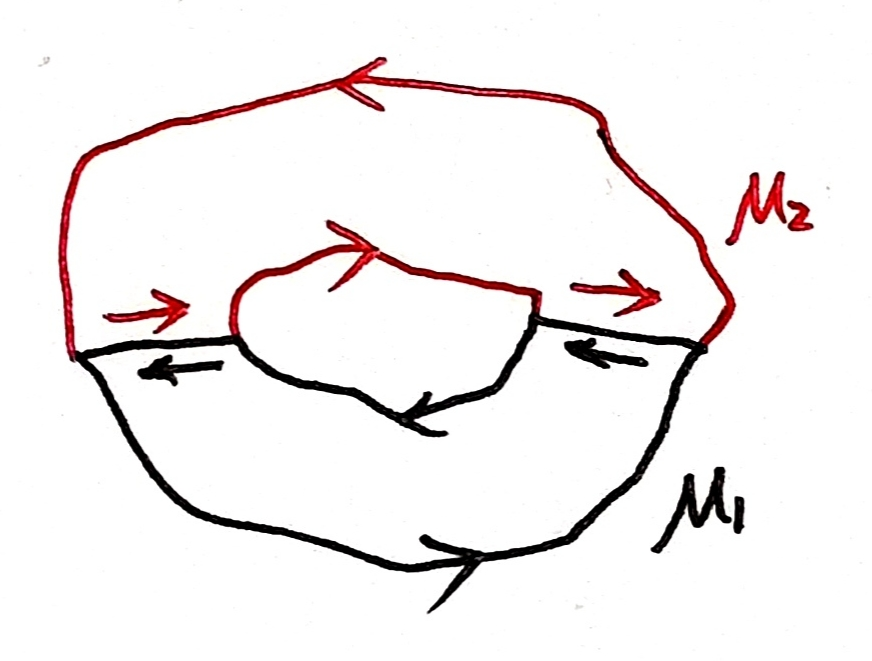
\includegraphics[width=0.3\textwidth]{figure/5.1-1} %图片的名称或者路径之中有空格会出问题 
			\caption{\textbf{Principle of contour deformation}} % 图片标题
			\label{pic 5.1-1}
		\end{figure}
	
		\vspace{2em}
		\begin{proof}
			\begin{align}
				\int_{\gamma_1}{f(z) dz} - \int_{\gamma_2}{f(z) dz} 
				&= \int_{\gamma_1}{f(z) dz} + \int_{\gamma_{2}^{-}}{f(z) dz} \\
				&= \int_{\mu_1}{f(z) dz} + \int_{\mu_2}{f(z) dz} = 0 + 0 = 0
			\end{align}
		\end{proof}	
	\end{thm}

	\vspace{2em}
	下面给出Thm \ref{thm 5.1.1} 的一种Special Case. (Interior($\gamma_1$)仅有一点不在$\Omega$ 内)
	\begin{corollary}\label{cor 5.1.2}
		Let $\Omega \subset \C$ be open, $f : \Omega \longrightarrow \C$ be holomorphic. Let $\gamma$ be a contour in $\Omega$ and $\exists \alpha \in Interior(\gamma)$, $\st Interior(\gamma) \backslash \{ \alpha \} \subset \C$. Then
		\begin{align}
			\int_{\gamma}{f(z) dz} = \int_{C_{r}(\alpha)}{f(z) dz} , \,\, where \,\, C_{r}(\alpha) \subset Interior(\gamma)
		\end{align}
	\end{corollary}
	
	\vspace{2em}
	下面给出更一般的表述.(Interior($\gamma$)内有有限个点不在$\Omega$ 内)
	\begin{corollary}\label{cor 5.1.3}
		Let $\Omega \subset \C$ be open, $f : \Omega \longrightarrow \C$ be holomorphic and $\gamma$ is a contour in $\Omega$. If $\alpha_1 , \cdots , \alpha_n \in Interior(\gamma)$, such $Interior(\gamma) \backslash \{ \alpha_1 , \cdots , \alpha_n \} \subset \Omega$, then
		\begin{align}
			\int_{\gamma}{f(z) dz} = \sum_{k = 1}^{n}{\int_{C_{r_k}(\alpha_k)}{f(z) dz}} 
		\end{align}
		where $C_{r_k}(\alpha_k)$ are disjoint “small” circles.
		
		\begin{figure}[htbp]  %h此处,t页顶,b页底,p独立一页,浮动体出现的位置
			\centering  %图表居中
			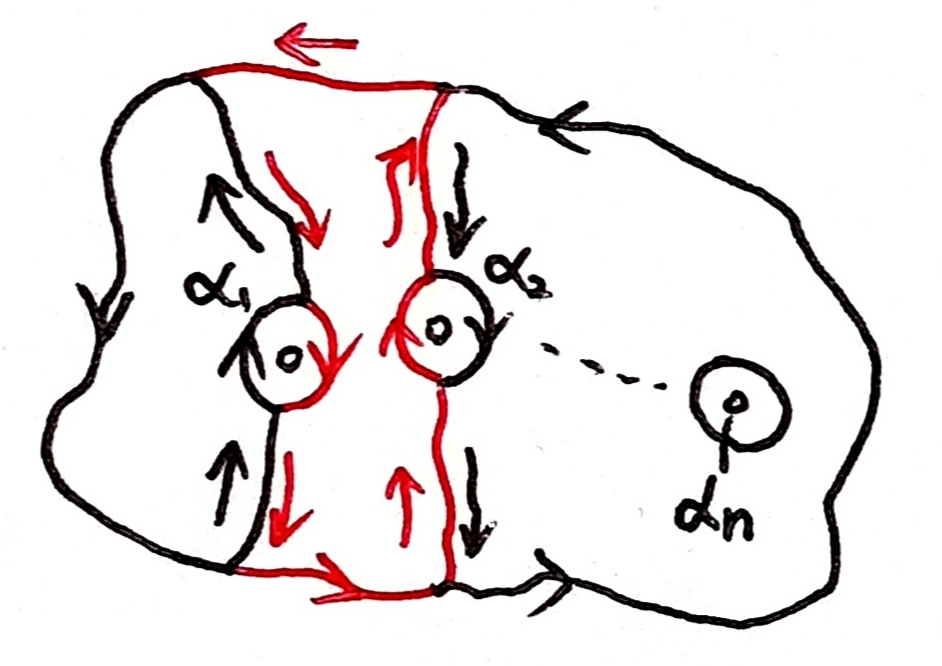
\includegraphics[width=0.3\textwidth]{figure/5.1-2} %图片的名称或者路径之中有空格会出问题 
			\caption{\textbf{Principle of contour deformation (Special Case)}} % 图片标题
			\label{pic 5.1-2}
		\end{figure}
	
		\begin{proof}
			即证
			\begin{align}
				\int_{\gamma}{f(z) dz} + \sum_{k = 1}^{n}{\int_{C_{r_k}^{-}(\alpha_k)}{f(z) dz}} = \sum_{k = 1}^{n}{\int_{\mu_{k}}{f(z) dz}} = \sum_{k = 1}^{n}{0} = 0
			\end{align}
		\end{proof}
	\end{corollary}

\newpage
\section{$Cauchy \,\, Integral \,\, Formulas$}
	\begin{center}
		接下来我们介绍另一个计算环路积分非常重要的公式——\textbf{Cauchy Integral Formulas}.
	\end{center}

\paragraph{Cauchy Integral Formulas}
	首先给出一个命题.
	\begin{proposition}\label{prop 5.2.1}
		Let $\Omega \subset \C$ be open, $f : \Omega \longrightarrow \C$ be holomorphic, $\gamma$ be a contour in $\Omega$. Assume $\exists \alpha \in Interior(\gamma)$, $\st$
		\begin{align}
			Interior(\gamma) \backslash \{ \alpha \} \subset \Omega \,\,\,\, and \,\,\,\, \lim_{z \to \alpha}{(z - \alpha)f(z)} = 0
		\end{align}
		Then
		\begin{align}
			\int_{\gamma}{f(z) dz} = 0
		\end{align}
	
		\vspace{2em}
		\begin{proof}
			$\forall \epsilon > 0$, $\exists \delta > 0$, $\st$
			\begin{align}
				\left| z - \alpha \right| < \delta \,\, \Rightarrow \,\, \left| (z - \alpha) f(z) \right| < \epsilon
			\end{align}
			By the \textbf{principle of contour deformation} (Thm \ref{thm 5.1.1}),
			\begin{align}
				\int_{\gamma}{f(z) dz} = \int_{C_{r}(\alpha)}{f(z) dz} , \,\, where \,\, 0 < r < \delta
			\end{align}
			Then
			\begin{align}
				\left| \int_{\gamma}{f(z) dz} \right| 
				\leq \sup_{z \in C_{r}(\alpha)}{\left| f(z) \right|} \cdot length(\gamma) 
				&= \sup_{z \in C_{r}(\alpha)}{\left| f(z) \right|} \cdot 2 \pi r \\
				&< \frac{\epsilon}{r} \cdot 2 \pi r = 2 \pi \epsilon
			\end{align}
		\end{proof}
	\end{proposition}

	\newpage
	下面给出\textbf{Cauchy Integral Formulas}.
	\begin{thm}\label{thm 5.2.1}
		\textbf{CIF}.\\
		Let $\Omega \subset \C$ be open, $f : \Omega \longrightarrow \C$ be holomorphic. Then for any $z_0 \in \Omega$,
		\begin{align}
			f(z_0) = \frac{1}{2 \pi i} \int_{\gamma}{\frac{f(\zeta)}{\zeta - z_0} d\zeta}
		\end{align}
		where $\gamma$ is any contour in $\Omega$ $\st$ $z_0 \in Interior(\gamma) \subset \Omega$.
		
		\vspace{2em}
		\begin{proof}
			Let
			\begin{align}
				g(z) = \frac{f(z) - f(z_0)}{z - z_0}
			\end{align}
			Then $g(z)$ is holomorphic on $\Omega \backslash \{ z_0 \}$. Clearly
			\begin{align}
				\lim_{z \to z_0}{(z - z_0) g(z)} = 0 , \,\, Interior(\gamma) \backslash \{ z_0 \} \subset \Omega \backslash \{ z_0 \}
			\end{align}
			By Prop \ref{prop 5.2.1},
			\begin{align}
				\int_{\gamma}{g(z) dz} = 0 \,\, \Rightarrow \,\, \int_{\gamma}{\frac{f(z)}{z - z_0} dz} = \int_{\gamma}{\frac{f(z_0)}{z - z_0} dz}
			\end{align}
			Therefore
			\begin{align}
				\int_{\gamma}{\frac{f(z)}{z - z_0} dz} 
				= \int_{\gamma}{\frac{f(z_0)}{z - z_0} dz} 
				= f(z_0) \int_{\gamma}{\frac{1}{z - z_0} dz} 
				&= f(z_0) \int_{C_{r}(z_0)}{\frac{1}{z - z_0} dz} \\
				&= 2 \pi i \cdot f(z_0)
			\end{align}
		\end{proof}
	\end{thm}

	\vspace{2em}
	Therefore, according to Cauchy Integral Formulas, we get
	\begin{align}
		f(z) = \frac{1}{2 \pi i} \int_{\gamma}{\frac{f(\zeta)}{\zeta - z} d\zeta} 
	\end{align}
	\begin{center}
		where $f$ is holomorphic on an open set containing the contour $\gamma$ and its interior, $z \in Interior(\gamma)$.
	\end{center}

	\newpage
\paragraph{高阶Cauchy Integral Formulas}
	下面给出\textbf{高阶}的Cauchy Integral Formulas.
	\begin{thm}\label{thm 5.2.2}
		Let $\Omega \subset \C$ be open, $f : \Omega \longrightarrow \C$ be holomorphic. Then $f$ is complex differentiable to all orders and moreover, $\forall z \in \Omega$
		\begin{align}
			f^{(n)}(z) = \frac{n!}{2 \pi i} \int_{\gamma}{\frac{f(\zeta)}{(\zeta - z)^{n + 1}} d\zeta} , \,\, n = 0 , 1 , 2 , \cdots
		\end{align}
		where $\gamma$ is any contour in $\Omega$ $\st$ $z \in Interior(\gamma) \subset \Omega$.
	\end{thm}

\vspace{2em}
\paragraph{\textbf{Cauchy's Inequalities}}
	作为\textbf{柯西积分公式 (CIF)}的推论,下面可得到\textbf{Cauchy's Inequalities}.
	\begin{corollary}\label{cor 5.2.3}
		\textbf{Cauchy's Inequalities}.\\
		If $f$ is holomorphic on an open set $\Omega$ with $D_{R}(z_0) \subset \Omega$, $R > 0$, then
		\begin{align}
			\left| f^{(n)}(z_0) \right| \leq \frac{n! \,\, \Vert f \Vert_{C_{R}(z_0)}}{R^n} , \,\, where \,\, \Vert f \Vert_{C_{R}(z_0)} = \sup_{z \in C_{R}(z_0)}{\left| f(z) \right|}
		\end{align}
	\end{corollary}

\vspace{2em}
\paragraph{\textbf{Liouville's therom}}
	下面给出\textbf{CIF} 的另一条重要推论. 在此之前,先给出\textbf{整函数 (entire)}的定义.
	\begin{defn}\label{def 5.2.1}
		A holomorphic function defined on the whole $\C$ is called an \underline{\textcolor{blue}{\textbf{entire function}}}.
	\end{defn}

	\vspace{2em}
	下面给出\textbf{刘维尔定理 (Liouville's theorem)}的内容.
	\begin{corollary}\label{cor 5.2.4}
		\textbf{Liouville's theorem}.
		\begin{center}
			If $f$ is entire and bounded, then $f$ is constant.
		\end{center}
		
		\vspace{2em}
		\begin{proof}
			$\forall z \in \C$, by \textbf{Cauchy's Inequalities (Cor \ref{cor 5.2.3})}
			\begin{align}
				\left| f^{'}(z) \right| \leq \frac{\Vert f \Vert_{\C}}{R} \leq \frac{M}{R} , \,\, where \,\, \left| f \right| \leq M
			\end{align}
			Letting $R \to \infty$, we get $f^{'}(z) = 0$, $\forall z \in \C$ $\,\, \Rightarrow \,\,$ $f$ is constant.
		\end{proof}
	\end{corollary}

\newpage
\paragraph{具有原函数的充要条件}
	下面在定理 \ref{thm 4.1.3} 的基础上,再增加一条具有原函数的充要条件.
	\begin{thm}\label{thm 5.2.5}
		Let $\Omega \subset \C$ be a region, $f : \Omega \longrightarrow \C$ be continuous. Then \textbf{TFAE} \\
		(the followings are equivalent):
		\begin{enumerate}
			\item[(1)]$f$ admits a primitive on $\Omega$.
			
			\item[(2)]$\forall \alpha , \beta \in \Omega$, $\int_{\gamma}{f(z) dz}$ is invariant for any path.
			
			\item[(3)]$\forall \alpha , \beta \in \Omega$, $\int_{\gamma}{f(z) dz}$ is invariant for any zig-zag path.
			
			\item[(4)]$\int_{\gamma}{f(z) dz} = 0$ for any closed path $\gamma \subset \Omega$. 
		\end{enumerate}
	
		\vspace{2em}
		\begin{proof}
			$(4) \Rightarrow (2)$: Fix $\alpha , \beta \in \Omega$, $\forall$ two paths $\gamma_1 , \gamma_2 \subset \Omega$ joining $\alpha$ to $\beta$, by (4)
			\begin{align}
				\int_{\gamma_1}{f(z) dz} - \int_{\gamma_2}{f(z) dz} = \int_{\gamma_1 \circ \gamma_{2}^{-}}{f(z) dz} = 0 , \,\, where \,\, \gamma_1 \circ \gamma_{2}^{-} \,\, is \,\, a  \,\, closed \,\, path \,\, in \,\, \Omega
			\end{align}
			Therefore
			\begin{align}
				\int_{\gamma_1}{f(z) dz} = \int_{\gamma_2}{f(z) dz} , \,\, \forall \gamma_1 , \gamma_2 \subset \Omega
			\end{align}
		\end{proof}
	\end{thm}

\vspace{2em}
\paragraph{\textbf{Morera's Theorem}}
	有了具有原函数的充要条件之后 (Thm \ref{thm 5.2.5}),下面我们可以对全纯函数进行充要刻画,此即为\textbf{Morera's Theorem} 的推广.
	
	\begin{proposition}\label{prop 5.2.2}
		Let $\Omega \subset \C$ be \textbf{simply connected}, $f : \Omega \longrightarrow \C$ be continuous. Then \textbf{TFAE}
		\begin{enumerate}
			\item[(1)]$f$ is holomorphic on $\Omega$.
			
			\item[(2)]$\int_{\gamma}{f(z) dz} = 0$ for any closed path $\gamma \subset \Omega$. 
		\end{enumerate}
		
		\vspace{1em}
		\begin{rmk}
			命题中$(2) \Rightarrow (1)$ 的部分即为\textbf{Morera's Theorem}.
		\end{rmk}
	
		\vspace{1em}
		\begin{proof}
			$(1) \Rightarrow (2)$: is by \textbf{Cauchy's Theorem} (Thm \ref{thm 4.3.2}). \\
			$(2) \Rightarrow (1)$: By Thm \ref{thm 5.2.5}, $f$ admits a primitive $F$ on $\Omega$, i.e. $F^{'} = f$, then $F$ is holomorphic on $\Omega$. \\
			By \textbf{CIF} (Thm \ref{thm 5.2.2}), $F$ is infinitely complex differentiable. \\
			In particular, $F$ is twice complex differentiable. $\Rightarrow$ $F^{''} = f^{'}$ $\Rightarrow$ $f$ is holomorphic on $\Omega$. 
		\end{proof}
	\end{proposition}

	\newpage
	由\textbf{命题 \ref{prop 5.2.2}}可直接得到如下推论.
	\begin{corollary}\label{cor 5.2.6}
		Every holomorphic function on a simply connected region admits a primitive.
	\end{corollary}

	\vspace{2em}
	在利用\textbf{命题 \ref{prop 5.2.2} (Morera's Thereom)}判定函数全纯时,要注意条件 (2)中道路$\gamma$ 的\textbf{任意性}. 下面便给出一个反例.
	\begin{example}\label{ex 5.2.1}
		Suppose $\int_{C_{r}(0)}{f(z) dz} = 0$ for all $0 < r < 1$, can we conclude $f$ is holomorphic on $\mathbb{D}$?
		
		\vspace{2em}
		\begin{solution}
			The answer is absolutely No. Take $f(z) = \left| z \right|^2$. Then $\int_{C_{r}(0)}{f(z) dz} = 0$, $\forall 0 < r < 1$. \\
			Since
			\begin{align}
				f(z) = \left| z \right|^2 = z \cdot \overline{z} , \,\, \frac{\partial f}{\partial \overline{z}} = z \neq 0 , \,\, \forall z \in \C \backslash \{ 0 \}
			\end{align}
			Therefore, $f$ is not holomorphic on $\mathbb{D}$.
			
			\begin{rmk}
				事实上,取道路$\gamma$ 为以原点为圆心,$\frac{1}{2}$ 为半径的上半圆,逆时针方向,可证$\int_{\gamma}{f(z) dz} \neq 0$.
			\end{rmk}
		\end{solution}
	\end{example}


	



\newpage
\section{课堂例题$2024-03-25$}
	\begin{enumerate}
		\item Evaluate 
		\begin{align}
			\int_{\gamma}{\frac{2z - 1}{z^2 - z} dz}
		\end{align}
		where $\gamma$ is any contour $\st$ $\overline{\mathcal{D}} \subset Interior(\gamma)$.
		
		\vspace{2em}
		\begin{solution}
			By Cor \ref{cor 5.1.3},(\textbf{闭路变形原理})
			\begin{align}
				\int_{\gamma}{f(z) dz} 
				&= \int_{C_{\frac{1}{3}}(0)}{f(z) dz} + \int_{C_{\frac{1}{3}}(1)}{f(z) dz} \\
				&= \int_{C_{\frac{1}{3}}(0)}{(\frac{1}{z - 1} + \frac{1}{z}) dz} + \int_{C_{\frac{1}{3}}(1)}{(\frac{1}{z - 1} + \frac{1}{z}) dz}
			\end{align}
			Since $\frac{1}{z - 1}$ is holomorphic on \textcolor{red}{$Interior(C_{\frac{1}{3}}(0)) = D_{\frac{1}{3}}(0)$}, where $D_{\frac{1}{3}}(0)$ is simply connected, then \\
			by Cauchy's Theorem,
			\begin{align}
				\int_{C_{\frac{1}{3}}(0)}{(\frac{1}{z - 1} + \frac{1}{z}) dz} = \int_{C_{\frac{1}{3}}(0)}{\frac{1}{z} dz}
			\end{align}
			Similarly, since $\frac{1}{z}$ is holomorphic on $D_{\frac{1}{3}}(1)$, then
			\begin{align}
				\int_{C_{\frac{1}{3}}(1)}{(\frac{1}{z - 1} + \frac{1}{z}) dz} = \int_{C_{\frac{1}{3}}(1)}{\frac{1}{z - 1} dz}
			\end{align}
			Therefore
			\begin{align}
				\int_{\gamma}{f(z) dz} 
				&= \int_{C_{\frac{1}{3}}(0)}{(\frac{1}{z - 1} + \frac{1}{z}) dz} + \int_{C_{\frac{1}{3}}(1)}{(\frac{1}{z - 1} + \frac{1}{z}) dz} \\
				&= \int_{C_{\frac{1}{3}}(0)}{\frac{1}{z} dz} + \int_{C_{\frac{1}{3}}(1)}{\frac{1}{z - 1} dz} \\
				&= 2\pi i + 2\pi i \\
				&= 4 \pi i
			\end{align}
		\end{solution}
		
		\newpage
		
		\item Evaluate
		\begin{align}
			&\int_{C_{3}(0)}{\frac{e^{z^2}}{z - 2} dz} \,\,\,\, ( = 2 \pi i f(z_0) = 2 \pi i e^4) \\
			&\int_{C_{1}(0)}{\frac{e^{z^2}}{z - 2} dz} \,\,\,\, ( = 0)
		\end{align}
	
		\vspace{2em}
		
		\item Evaluate
		\begin{align}
			\int_{C_{2}(0)}{\frac{\sin{z}}{z^2 + 1} dz}
		\end{align}
		
		\vspace{2em}
		\begin{solution}
			\begin{align}
				\int_{C_{2}(0)}{\frac{\sin{z}}{z^2 + 1} dz} 
				&= \int_{C_{\frac{1}{2}}(i)}{\frac{\sin{z}}{z + i} \cdot \frac{1}{z - i} dz} + \int_{C_{\frac{1}{2}}(-i)}{\frac{\sin{z}}{z - i} \cdot \frac{1}{z + i} dz} \\
				&= 2 \pi i \cdot \frac{\sin{i}}{2i} + 2 \pi i \cdot \frac{\sin{(-i)}}{-2i} \\
				&= 2\pi \sin{i}
			\end{align}
		\end{solution}
	
		\vspace{2em}
		
		\item Evaluate
		\begin{align}
			\int_{C_{3}(0)}{\frac{z}{(z - 1)(z - 2)^2} dz}
		\end{align}
	
		\vspace{2em}
		\begin{solution}
			By Thm \ref{thm 5.2.2} (高阶Cauchy Integral Formulas),
			\begin{align}
				\int_{C_{3}(0)}{\frac{z}{(z - 1)(z - 2)^2} dz} 
				&= \int_{C_{\frac{1}{3}}(1)}{\frac{z}{(z - 2)^2} \cdot \frac{1}{z - 1} dz} + \int_{C_{\frac{1}{3}}(2)}{\frac{z}{z - 1} \cdot \frac{1}{(z - 2)^2} dz} \\
				&= 2 \pi i + 2 \pi i \left( \frac{z}{z - 1} \right)^{'}\Big|_{z = 2} \\
				&= 0
			\end{align}
		\end{solution}
	
		\vspace{1em}
		
		\item 课本第二章练习$T6$.
	\end{enumerate}

\newpage

\section{$Sequence \,\, of \,\, functions$}
\paragraph{概念}
	这一节我们来介绍有关复数域上函数列的相关概念和性质. 先回顾函数列收敛的定义.
	\begin{defn}\label{def 5.4.1}
		Let $\Omega \subset \C$ be open, $\{ f_n : \Omega \longrightarrow \C \}_{n = 1}^{\infty}$ be a sequence of function. \\
		We say $\{ f_n \}_{n = 1}$ \underline{\textcolor{blue}{\textbf{converges}}} if $\forall z \in \Omega$, $\{ f_{n}(z) \}_{n = 1}^{\infty}$ converges.\\
		We say $\{ f_n \}_{n = 1}^{\infty}$ \underline{\textcolor{blue}{\textbf{converges uniformly}}} if $\forall \epsilon > 0 , \exists N \in \N , \st$
		\begin{center}
			$m , n > N \,\, \Rightarrow \,\, \left| f_{m}(z) - f_{n}(z) \right| < \epsilon , \,\, \forall z \in \Omega$
		\end{center}
		We say $\{ f_n \}_{n = 1}^{\infty}$ \underline{\textcolor{blue}{\textbf{uniformly converges to $f$}}} if $\forall \epsilon > 0 , \exists N \in \N , \st$
		\begin{center}
			$n > N \,\, \Rightarrow \,\, \left| f_{n}(z) - f(z) \right| < \epsilon , \,\, \forall z \in \Omega$
		\end{center}
	\end{defn}
	
	\vspace{2em}
	下面给出一个经典的收敛但不一致收敛的例子.
	\begin{example}\label{ex 5.4.1}
		$\{ f_{n}(z) = z^n \}_{n = 1}^{\infty}$ on $\mathbb{D}$ is convergent but not uniformly convergent. However, the sequence is uniformly convergent on any compact subset on $\mathbb{D}$.
	\end{example}

\vspace{2em}
\paragraph{一致收敛}
	下面给出函数列一致收敛的性质,即\textbf{积分与极限可交换次序}.
	\begin{thm}\label{thm 5.4.1}
		Let $\Omega \subset \C$ be open, $\{ f_n : \Omega \longrightarrow \C \}_{n = 1}^{\infty}$ be a sequence of continuous functions that converges uniformly to $f$ \textbf{on every compact subset of $\Omega$}. Then
		\begin{enumerate}
			\item[(1)]$f$ is continuous.
			
			\vspace{1em}
			
			\item[(2)]If $\gamma \subset \Omega$ is a path with finite length, then
			\begin{align}
				\lim_{n \to \infty}{\int_{\gamma}{f_{n}(z) dz}} = \int_{\gamma}{f(z) dz}
			\end{align}
		
			\vspace{1em}
			
			\item[(3)]If $f_n$ is holomorphic for all $n$, then so is $f$. Moreover, \\
			$\{ f_{n}^{'} \}_{n = 1}^{\infty}$ converges uniformly to $f^{'}$ \textbf{on every compact subset of $\Omega$}.
		\end{enumerate}
		
		\vspace{1em}
		\begin{rmk}
			性质 (2)即说明了对于一致收敛的函数列,\textbf{极限与积分可交换次序},即
			\begin{align}
				\lim_{n \to \infty}{\int_{\gamma}{f_{n}(z) dz}} = \int_{\gamma}{\lim_{n \to \infty}{f_{n}(z) dz}} = \int_{\gamma}{f(z) dz}
			\end{align}
		\end{rmk}
	
		\newpage
		\begin{proof}
			\begin{enumerate}
				\item[(1)]: Fix $z_0 \in \Omega$, $\forall \epsilon > 0$\\
				Since $\{f_n\}_{n = 1}^{\infty}$ converges uniformly to $f$, there exists $N \in \N$, $\st$
				\begin{align}
					\left| f(z) - f_{n}(z) \right| \leq \epsilon , \,\, \forall n \geq N , \forall z \in \Omega
				\end{align}
				Since $f_N$ is continuous at $z_0$, there exist $\delta > 0$, $\st$
				\begin{align}
					\left| f_{n}(z) - f_{n}(z_0) \right| \leq \epsilon , \,\, \forall z \in D_{\delta}(z_0)
				\end{align}
				Therefore
				\begin{align}
					\left| f(z) - f(z_0) \right| 
					&\leq \left| f(z) - f_{N}(z) \right| + \left| f_{N}(z) - f_{N}(z_0) \right| + \left| f_{N}(z_0) - f(z_0) \right| \\
					&\leq 3 \epsilon , \,\, \forall z \in D_{\delta}(z_0)
				\end{align}
				
				\vspace{2em}
				
				\item[(2)]: Fix $\epsilon > 0$. For any path $\gamma$ with finite length, $\gamma \subset \Omega$ is a compact subset of $\Omega$.\\
				Let $L = length(\gamma)$. Since $\{ f_n \}_{n = 1}^{\infty}$ converges uniformly on compact subset $\gamma$, $\exists N \in \N$, $\st$
				\begin{align}
					\left| f_{n}(z) - f(z) \right| \leq \frac{\epsilon}{L} , \,\, \forall z \in \gamma , \forall n > N
				\end{align}
				Hence, for all $n > N$,
				\begin{align}
					\left| \int_{\gamma}{f_{n}(z) dz} - \int_{\gamma}{f(z) dz} \right| \leq \int_{\gamma}{\left| f_{n}(z) - f(z) \right|} \leq \frac{\epsilon}{L} \cdot L = \epsilon , \,\, \forall n > N
				\end{align}
				Therefore
				\begin{align}
					\lim_{n \to \infty}{\int_{\gamma}{f_{n}(z) dz}} = \int_{\gamma}{f(z) dz} = \int_{\gamma}{\lim_{n \to \infty}{f_{n}(z) dz}}
				\end{align}
			
				\vspace{2em}
				\item[(3)]: 下面分两部分证明. (对应书\footnote{课堂教材:\textbf{《$Complex \,\, Analysis$》---  $Elias \,\, M. \,\, Stein$}}P54 Thm 5.3)
				\begin{itemize}
					\item $f$ is holomorphic. \\
					$\forall \alpha \in \Omega$, $\exists r > 0$, $\st D_{r}(\alpha) \subset \Omega$. Let $\gamma$ be any closed path in $D_{r}(\alpha)$.\\
					Since $f_n$ is holomorphic on $D_{r}(\alpha)$, by \textbf{Cauchy's Theorem (Thm \ref{thm 4.3.2})}, 
					\begin{align}
						\int_{\gamma}{f_{n}(z) dz} = 0
					\end{align}
					By (2) proofed previously, 
					\begin{align}
						\int_{\gamma}{f(z) dz} = \lim_{n \to \infty}{\int_{\gamma}{f_{n}(z) dz}} = 0
					\end{align}
				
					\newpage
					By \textbf{Morera's Theorem (Prop \ref{prop 5.2.2})}, $f$ is holomorphic on $D_{r}(\alpha)$.\\
					In particular, $f$ is complex differentiable at $\alpha$. Since $\alpha$ is arbitrary, $f$ is holomorphic on $\Omega$.
					
					\vspace{2em}
					
					\item $\{ f_{n}^{'} \}_{n = 1}^{\infty}$ converges uniformly to $f^{'}$ on every compact subset of $\Omega$. \\
					$\forall z_0 \in \Omega$, $\exists r > 0$, $\st \overline{D}_{r}(z_0) \subset \Omega$. \\
					Since $f_n \longrightarrow f$ converges uniformly on $C_{r}(z_0)$, we have $\forall z \in D_{\frac{r}{2}}(z_0)$
					\begin{align}
						\frac{f_{n}(\zeta)}{(\zeta - z)^2} \to \frac{f(\zeta)}{(\zeta - z)^2} \,\, uniformly \,\, on \,\, C_{r}(z_0)
					\end{align}
					i.e. $\forall \epsilon > 0$, $\exists N \in \N$, $\st$
					\begin{align}
						\left| \frac{f_{n}(\zeta)}{(\zeta - z)^2} - \frac{f(\zeta)}{(\zeta - z)^2} \right| < \frac{\epsilon}{r}, \,\, \forall n > N , \forall \zeta \in C_{r}(z_0)
					\end{align}
					Therefore
					\begin{align}
						\left| f_{n}^{'}(z) - f^{'}(z) \right| 
						&= \left| \frac{1}{2\pi i} \int_{C_{r}(z_0}{\left( \frac{f_{n}(\zeta)}{(\zeta - z)^2} - \frac{f(\zeta)}{(\zeta - z)^2} \right) d\zeta} \right| \\
						&< \frac{1}{2 \pi i} \cdot \frac{\epsilon}{r} \cdot 2 \pi r i \\
						&= \epsilon , \,\, \forall n > N , \forall z \in D_{\frac{r}{2}}(z_0)
					\end{align}
					It tells $f_{n}^{'} \to f^{'}$ uniformly on $D_{\frac{r}{2}}(z_0)$. \\
					For any compact subset $K \subset \Omega$, consider the open covering $\{ D_{\frac{1}{2} r_x}(x) \subset \Omega \}_{x \in K}$.\\
					There exists a finite subcovering $K \subset \{ D_{r_i}(x_i) \subset \Omega \}_{i = 1}^{n}$. \\
					We can proof $f_{n}^{'} \to f^{'}$ uniformly on $K$.
				\end{itemize}
			\end{enumerate}
		\end{proof}
	\end{thm}

\newpage

\section{课堂例题$2024-03-29$}
	\begin{enumerate}
		\item Evaluate 
		\begin{align}
			\int_{C_{3}(0)}{\frac{z}{(z - 1)(z - 2)^2} dz}
		\end{align}
	
		\vspace{2em}
		\begin{solution}
			\begin{align}
				\int_{C_{3}(0)}{\frac{z}{(z - 1)(z - 2)^2} dz}
				&= \int_{C_{\frac{1}{3}}(0)}{\frac{z}{(z - 2)^2} \cdot \frac{1}{z - 1} dz} + \int_{C_{\frac{1}{3}}(2)}{\frac{z}{z - 1} \cdot \frac{1}{(z - 2)^2} dz} \\
				&= 2\pi i + 2\pi i \left( \frac{z}{z - 1} \right)^{'} \Big|_{z = 2} \\
				&= 0
			\end{align}
		\end{solution}
	\end{enumerate}

\chapter{$Week \,\, 6$}
\section{课堂例题$2024-04-01$}
	\begin{center}
		本节为习题课. (博士研究生助教代课)
	\end{center}
	\begin{enumerate}
		\item 课本第二章练习$T1 , T2 , T3 , T4$.
	\end{enumerate}

\newpage

\section{函数项级数,全纯函数解析}
\paragraph{回顾}
	在介绍复数域上函数项级数的性质之前,先回顾一下函数列的性质 (Thm \ref{thm 5.4.1}).
	\begin{thm}\label{thm 6.2.1}
		\textbf{一致收敛 $\Rightarrow$ 积分与极限可交换次序}.\\
		Let $\Omega \subset \C$ be open, $\{ f_n : \Omega \longrightarrow \C \}_{n = 1}^{\infty}$ be a sequence of continuous functions that converges uniformly to $f$ \textbf{on every compact subset of $\Omega$}. Then
		\begin{enumerate}
			\item[(1)]$f$ is continuous.
			
			\vspace{1em}
			
			\item[(2)]If $\gamma \subset \Omega$ is a path with finite length, then
			\begin{align}
				\lim_{n \to \infty}{\int_{\gamma}{f_{n}(z) dz}} = \int_{\gamma}{f(z) dz}
			\end{align}
			
			\vspace{1em}
			
			\item[(3)]If $f_n$ is holomorphic for all $n$, then so is $f$. Moreover, \\
			$\{ f_{n}^{'} \}_{n = 1}^{\infty}$ converges uniformly to $f^{'}$ \textbf{on every compact subset of $\Omega$}.
		\end{enumerate}
		
		\vspace{1em}
		\begin{rmk}
			\begin{itemize}
				\item 事实上,结论 (3)可做推广,即当函数列$\{ f_n \}_{n = 1}^{\infty}$ 满足上述条件时,有:
				\begin{center}
					$\{ f_{n}^{(k)} \}_{n = 1}^{\infty}$ converges uniformly to $f^{(k)}$ \textbf{on every compact subset of $\Omega$}.
				\end{center}
			
				\vspace{2em}
				
				\item 注意实变函数列与复变函数列的\textbf{可微性}的区别,即实变函数列不满足定理中的 (3). 下面给出结论 (3)在实变函数列下的反例.
				
				\vspace{1em}
				
				\begin{example}\label{ex 6.2.1}
					Let $f_{n}(x) = \sqrt{x^2 + \frac{1}{n}}$, $x \in [-1 , 1]$. Then $\{ f_n \}_{n = 1}^{\infty}$ converges uniformly to $f(x) = \left| x \right|$. \\
					Though $f_n$, $n = 1 , 2 , \cdots$ are differentiable over $[-1 , 1]$, the limit function $f(x) = \left| x \right|$ is \textbf{not differentiable} at $x = 0$.
				\end{example}
			\end{itemize}
		\end{rmk}
	
		\vspace{2em}
		\begin{proof}
			详见定理 \ref{thm 5.4.1}证明.
		\end{proof}
	\end{thm}

\newpage

\paragraph{函数项级数}
	下面给出函数项级数收敛的定义.
	\begin{defn}\label{def 6.2.1}
		Let $\Omega \subset \C$ be open, $\{ f_n : \Omega \longrightarrow \C \}_{n = 1}^{\infty}$ be a sequence of functions. \\
		We say $\overset{\infty}{\underset{n = 1}{\sum}}{f_n}$ \underline{\textcolor{blue}{\textbf{converges}}} if $\{ S_{N} = \overset{N}{\underset{n = 1}{\sum}}{f_n} \}_{N = 1}^{\infty}$ converges.  \\
		We say $\overset{\infty}{\underset{n = 1}{\sum}}{f_n}$ \underline{\textcolor{blue}{\textbf{converges uniformly}}} if $\{ S_{N} = \overset{N}{\underset{n = 1}{\sum}}{f_n} \}_{N = 1}^{\infty}$ converges uniformly).
	\end{defn}

	\vspace{2em}
	下面给出判断函数项级数一致收敛性的经典方法 (\textbf{Weierstrass M-test}).
	
	\begin{proposition}\label{prop 6.2.1}
		\textbf{Weierstrass M-test}. \\
		If $\left| f_{n}(z) \right| \leq M_n$, $n = 1 , 2 , \cdots , \forall z \in \Omega$, and $\overset{\infty}{\underset{n = 1}{\sum}}{M_n} < \infty$, then $\overset{\infty}{\underset{n = 1}{\sum}}{f_n}$ converges uniformly.
		
		\vspace{2em}
		\begin{proof}
			Let $S_N = \overset{N}{\underset{n = 1}{\sum}}{f_n}$, $\forall N \in \N$. Since $\overset{\infty}{\underset{n = 1}{\sum}}{M_n} < \infty$, then\\
			$\forall \epsilon > 0 , \exists N \in \N , \st n > m > N$
			\begin{align}
				\left| S_n - S_m \right| = \left| f_{n}(z) + \cdots + f_{m + 1}(z) \right| \leq \sum_{j = m + 1}^{\infty}{M_j} \leq \epsilon , \,\, \forall z \in \Omega
			\end{align}
			Therefore, $\{ S_n \}_{n = 1}^{\infty}$ converges uniformly. $\,\, \Rightarrow \,\,$ $\{ f_n \}_{n = 1}^{\infty}$ converges uniformly.
		\end{proof}
	\end{proposition}

\vspace{2em}
\paragraph{解析与全纯等价}
	下面证明\textbf{全纯}函数均\textbf{解析 (可展成幂级数)}. 
	\begin{center}
		\textbf{(该定理与定理 \ref{thm 3.1.2}共同说明了,解析 $\Leftrightarrow$ 全纯)}
	\end{center}
	\begin{thm}\label{thm 6.2.2}
		Suppose $f$ is holomorphic on an open set $\Omega \subset \C$. Then $\forall z_0 \in \Omega$ with $D_{r}(z_0) \subset \Omega$ for some $r > 0$, $f$ has a power series expansion at $z_0$.
		\begin{align}
			f(z) = \sum_{n = 0}^{\infty}{a_n (z - z_0)^n} , \,\, \forall z \in D_{r}(z_0)
		\end{align}
		$where \,\, a_n = \frac{f^{(n)}(z_0)}{n!} , \,\, \forall n \geq 0$.\\
		
		\begin{proof}
			Fix $z \in D_{r}(z_0)$. By \textbf{CIF (Thm \ref{thm 5.2.1})},
			\begin{align}
				f(z) = \frac{1}{2\pi i}\int_{C_{r}(z_0)}{\frac{f(\zeta)}{\zeta - z} d\zeta}
			\end{align}
			Then
			\begin{align}
				\frac{1}{\zeta - z} 
				= \frac{1}{\zeta - z_0 - (z - z_0)} 
				= \frac{1}{\zeta - z_0} \cdot \frac{1}{1 - \frac{z - z_0}{\zeta - z_0}} 
			\end{align}
			Since $z \in D_{r}(z_0)$ is fixed, and $\forall \zeta \in C_{r}(z_0)$, there exists $0 < r < 1$, $\st$
			\begin{align}
				\left| \frac{z - z_0}{\zeta - z_0} \right| < r
			\end{align}
			Therefore,
			\begin{align}
				\sum_{n = 0}^{N}{\left( \frac{z - z_0}{\zeta - z_0} \right)^n} \,\, \Rightarrow \,\, \frac{1}{1 - \frac{z - z_0}{\zeta - z_0}} , \,\, N \to \infty , \,\, \forall \zeta \in C_{r}(z_0)
			\end{align}
			converges uniformly \textbf{w.r.t. (with respect to , 关于)} $\zeta \in C_{r}(z_0)$. i.e.
			\begin{align}
				\sum_{n = 0}^{\infty}{\left( \frac{z - z_0}{\zeta - z_0} \right)^n} = \frac{1}{1 - \frac{z - z_0}{\zeta - z_0}} , \,\, \forall \zeta \in C_{r}(z_0)
			\end{align}
			Let
			\begin{align}
				g_{N}(\zeta)
				&= \sum_{n = 0}^{N}{\left( f(\zeta) \cdot \frac{1}{\zeta - z_0} \cdot \left( \frac{z - z_0}{\zeta - z_0} \right)^n \right)} \\
				&= f(\zeta) \cdot \frac{1}{\zeta - z_0} \sum_{n = 0}^{N}{\left( \frac{z - z_0}{\zeta - z_0} \right)^n} , \,\, \zeta \in C_{r}(z_0)
			\end{align}
			Then we have
			\begin{align}
				g_{N} \,\, &\Rightarrow \,\, f(\zeta) \cdot \frac{1}{\zeta - z_0} \cdot \frac{1}{1 - \frac{z - z_0}{\zeta - z_0}} \\
				&= \frac{f(\zeta)}{\zeta - z} , \,\, N \to \infty , \,\, \zeta \in C_{r}(z_0)
			\end{align}
			converges uniformly w.r.t. $\zeta \in C_{r}(z_0)$. Therefore, by Thm \ref{thm 6.2.1},
			\begin{align}
				f(z) 
				= \frac{1}{2\pi i}\int_{C_{r}(z_0)}{\frac{f(\zeta)}{\zeta - z} d\zeta}
				&= \frac{1}{2\pi i} \int_{C_{r}(z_0)}{\lim_{N \to \infty}{g_{N}(\zeta) d\zeta}} \\
				&= \lim_{N \to \infty}{\frac{1}{2 \pi i} \int_{C_{r}(z_0)}{g_{N}(\zeta) d\zeta}} \\
				&= \lim_{N \to \infty}{\frac{1}{2 \pi i} \int_{C_{r}(z_0)}{ \left( f(\zeta) \cdot \frac{1}{\zeta - z_0} \sum_{n = 0}^{N}{\left( \frac{z - z_0}{\zeta - z_0} \right)^n } \right) d\zeta } } \\
				&= \lim_{N \to \infty}{\sum_{n = 0}^{N} \frac{1}{2 \pi i} \int_{C_{r}(z_0)}{ \left( f(\zeta) \cdot \frac{1}{\zeta - z_0} \left( \frac{z - z_0}{\zeta - z_0} \right)^n \right) d\zeta } } \\
				&= \sum_{n = 0}^{\infty} \left( \frac{1}{2 \pi i} \int_{C_{r}(z_0)}{ \frac{f(\zeta)}{(\zeta - z_0)^{n + 1}} d\zeta } \right) (z - z_0)^n \\
				&= \sum_{n = 0}^{\infty}{a_n (z - z_0)^n}
			\end{align}
			By \textbf{CIF (Thm \ref{thm 5.2.2})}, we have
			\begin{align}
				a_n = \frac{1}{2 \pi i} \int_{C_{r}(z_0)}{ \frac{f(\zeta)}{(\zeta - z_0)^{n + 1}} d\zeta } = \frac{f^{(n)}(z_0)}{n!} , \,\, \forall n \geq 0
			\end{align}
		\end{proof}
	
		\begin{rmk}
			事实上,该定理也提供了\textbf{CIF 高阶形式 (Thm \ref{thm 5.2.2})} 的另一种证明 (比较系数可得).
		\end{rmk}
	\end{thm}

\newpage

\section{解析延拓}
\paragraph{定义}
	下面先给出\textbf{解析延拓 (Analytic continuation)}的定义.
	\begin{defn}\label{def 6.3.1}
		Suppose $f$ and $F$ are holomorphic in nonempty regions $\Omega$ and $\hat{\Omega}$ respectively with $\Omega \subset \hat{\Omega}$. If $f(z) = F(z)$ in $\Omega$, then we say $F$ is an \underline{\textcolor{blue}{\textbf{analytic continuation}}} of $f$ in $\hat{\Omega}$.
	\end{defn}

\vspace{2em}
\paragraph{解析延拓的唯一性}
	在说明这之前,先给出一个有关全纯函数的非常重要的结论.
	
	\begin{thm}\label{thm 6.3.1}
		Suppose $f$ is holomorphic in a region $\Omega$ that vanishes on a sequence of distinct points with a limit in $\Omega$. Then $f(z) \equiv 0$ for all $z \in \Omega$.
		
		\vspace{1em}
		\begin{rmk}
			该定理说明了,不恒为零的全纯函数的\textbf{零点均为孤立点} (不为聚点).
		\end{rmk}
	
		\vspace{1em}
		\begin{proof}
			反证法. Suppose $\{ w_k \}_{k = 1}^{\infty} \subset \Omega$ with $\underset{k \to \infty}{\lim}{w_k} = z_0 \in \Omega$ and $f(w_k) = 0$, $k = 1 , 2 , \cdots$. \\
			Since $f$ is holomorphic in $\Omega$, $\forall z \in D_{r}(z_0)$
			\begin{align}
				f(z) = \sum_{n = 0}^{\infty}{a_n (z - z_0)^n} , \,\, for \,\, some \,\, r > 0
			\end{align}
			下面分为两步证明.
			\begin{itemize}
				\item We first show $f(z) \equiv 0$ on $D_{r}(z_0)$. \\
				Assume $f(z) \neq 0$ for $z \in D_{r}(z_0)$, then $\exists$ smalledt integer $m$ $\st$ $a_m \neq 0$. Now
				\begin{align}
					f(z) = a_m (z - z_0)^m (1 + g(z)) , \,\, where \,\, g(z) = \sum_{n = m + 1}^{\infty}{a_n (z - z_0)^{n - m}}
				\end{align}
				Since $g(z) \to 0$ as $z \to z_0$, $\forall \epsilon < 1$, there exists $\delta > 0$, $\st$
				\begin{align}
					\left| g(z) \right| \leq \epsilon < 1 , \,\, \forall z \in D_{\delta}^{*}(z_0)
				\end{align}
				Since $w_k \to z_0 \in \Omega$, $\exists k_0 \in \N$, $\st$ $w_{k_0} \in D_{\delta}^{*}(z_0)$. Then
				\begin{align}
					f(w_{k_0}) = a_m (z - z_0)^m (1 + g(w_{k_0})) \neq 0
				\end{align}
				which is a contradiction with that $f(w_{k_0}) = 0$.
				
				\item Then we shall show $f \equiv 0$ on $\Omega$. \\
				Let $U$ be the interior of $\{ z \in \Omega \mid f(z) = 0 \}$. Since $f(z) \equiv 0 , \forall z \in D_{r}(z_0)$, $U \neq \varnothing$ and $U$ is open. \\
				Moreover, 下面我们证明 $U$ is closed.
				\begin{itemize}
					\item For all $\{ z_k \}_{k = 1}^{\infty} \subset U$ with $z_k \to p \in \Omega$. 与第一步证明相同,可以得到\\
					$\exists r_p > 0$, $\st$ $f(z) \equiv 0 , \forall z \in D_{r_p}(p)$. 于是$p \in U$. 即$U$ 包含了自身序列的所有极限点. \\
					which means that $U$ is closed.
				\end{itemize}
				Therefore, $U \subset \Omega$ is both open and closed. Since $U \neq \varnothing$ and $\Omega$ is connected, then $U = \Omega$, \\
				which means $f \equiv 0$ on $\Omega$.
			\end{itemize}
		\end{proof}
	\end{thm}
	
	\vspace{2em}
	通过上述定理可得到,全纯函数的取值只由区域上\textbf{可数个点}决定.
	\begin{corollary}\label{cor 6.3.2}
		Suppose $f , g$ are holomorphic in a region $\hat{\Omega}$ and $f(z) = g(z)$ for all $z \in \Omega$, where $\Omega$ is an open subset of $\hat{\Omega}$. Then $f(z) = g(z)$ for $z \in \hat{\Omega}$.
	\end{corollary}

	\vspace{2em}
	By Cor \ref{cor 6.3.2},我们得到解析延拓若存在,则\textbf{必唯一}.
	\begin{corollary}\label{cor 3.3.3}
		Suppose $F$ and $G$ are both analytic continuation of $f$ into $\hat{\Omega}$. Then
		\begin{center}
			$F = G$ in $\hat{\Omega}$
		\end{center}
	\end{corollary}

\newpage

\section{对称原理}
\paragraph{引入}
	在实分析中,我们曾探讨过有关\textbf{连续函数的延拓 (Tietze 延拓定理}). 
	
	但在复分析中,对于\textbf{全纯函数的延拓}似乎不再那么容易与显然,因为全纯函数不仅要求在复平面上光滑,而且还具有一些 additional characteristically rigid properties. 
	\begin{center}
		(书P67 Problem 1. 给出了无法 (解析)延拓至$\overline{\mathbb{D}}$ 的定义在$\mathbb{D}$ 上的全纯函数.)
	\end{center}
	而本节将给出一种十分有用的情况下全纯函数的延拓,即在\textbf{关于实轴对称}的区域上的延拓.
	
\vspace{2em}
\paragraph{对称原理}
	为了讨论的方便,接下来的命题将默认以下几个记号:
	\begin{itemize}
		\item Let $\Omega$ be an open subset of $\C$ that is \textbf{symmetric} w.r.t. the real axis.
		
		\item Let $\Omega^{+}$ denote the part of $\Omega$ that lies in the upper half-plane and $\Omega^{-}$ the part that lies in the lower half-plane.
	\end{itemize}
	
	\vspace{2em}
	下面给出对称原理.
	\begin{thm}\label{thm 6.4.1}
		\textbf{Symmetric principle}. \\
		If $f^{+}$ and $f^{-}$ are holomorphic in $\Omega^{+}$ and $\Omega^{-}$ respectively that extends continuously to $I$ ($I = \Omega \cap \R$) and $f^{+}(x) = f^{-}(x)$ for all $x \in I$. Then
		\begin{align}
			f(z) = 
			\begin{cases}
				f^{+}(z) , z \in \Omega^{+} \\
				f^{+}(z) = f^{-}(z) , z \in I \\
				f^{-}(z) , z \in \Omega^{-}
			\end{cases}
		\end{align}
		is holomorphic in $\Omega$.
		
		\vspace{2em}
		\begin{proof}
			详见书P58 Thm 5.5 证明.
		\end{proof}
	\end{thm}

\newpage
\paragraph{\textbf{Schwartz} 反射原理}
	有了上述对称原理的铺垫后,下面给出全纯函数在\textbf{关于实轴对称}区域上的延拓定理. (\textbf{Schwartz 反射原理})
	\begin{thm}\label{thm 6.4.2}
		\textbf{Schwartz reflection principle}. \\
		Suppose $f$ is holomorphic in $\Omega^{+}$ that extends continuously to $I$ and $f$ is real-valued on $I$. Then $\exists F$ holomorphic in all $\Omega$, $\st$ $F = f$ in $\Omega^{+}$.
		
		\vspace{2em}
		\begin{proof}
			Define $f^{-}(z) = \overline{f(\overline{z})}$ for $z \in \Omega^{-}$. Fix $z_0 \in \Omega^{-} , \exists r > 0 , \st D_{r}(z_0) \subset \Omega^{-}$.\\
			Then $\overline{z_0} \in \Omega^{+}$ and $D_{r}(\overline{z_0}) \subset \Omega^{+}$. $\forall x \in D_{r}(z_0)$, $\overline{x} \in D_{r}(\overline{z_0})$\\
			Since $f$ is holomorphic in $\Omega^{+}$, by Thm \ref{thm 6.2.2} (全纯函数均解析)
			\begin{align}
				f(\overline{z}) = \sum_{n = 0}^{\infty}{a_n (\overline{z} - \overline{z_0})^n} , \,\, \forall \overline{z} \in D_{r}(\overline{z_0})
			\end{align}
			Then we have
			\begin{align}
				f^{-}(z) = \sum_{n = 0}^{\infty}{\overline{a_n} (z - z_0)^n} = \sum_{n = 0}^{\infty}{a_n (z - z_0)^n} , \,\, \forall z \in D_{r}(z_0)
			\end{align}
			Therefore, $f^{-}$ is analytic in $\omega^{-}$. By Thm \ref{thm 3.1.2}, $f^{-}$ is holomorphic in $\Omega^{-}$. (解析函数均全纯)\\
			Therefore, by \textbf{Symmetric principle (对称原理)}, 
			\begin{align}
				F(z) = 
				\begin{cases}
					f^{+}(z) , z \in \Omega^{+} \\
					f^{+}(z) = f^{-}(z) , z \in I \\
					f^{-}(z) , z \in \Omega^{-}
				\end{cases}
			\end{align}
			is holomorphic in $\Omega$.
		\end{proof}
	\end{thm}

\newpage

\section{课堂例题$2024-04-07$}
\begin{enumerate}
	\item \textbf{(课本P66 Ex10.)}\\
	Weierstrass's theorem states that a continuous function on $[0 , 1]$ can be uniformly approxiamted by polynomials. \textbf{Can every continuous function on the closed unit disc be approxiated uniformly by polynomials in the variable $z$?}
	
	\vspace{2em}
	
	\begin{solution}
		Absolutely No. Take $f(z) = \left| z \right|$ continuous on $\mathbb{D}$ into consideration. \\
		If there exists polynomials $\{ f_n \}_{n = 1}^{\infty}$, $\st$ $f_n \Rightarrow f$, then by Thm \ref{thm 6.2.1}, \\
		$f$ is holomorphic on $\mathbb{D}$, which is a contradiction with that $f$ is not differentiable at $x = 0$.
	\end{solution}

	\vspace{2em}
	
	\item Suppose $f$ is entire and real-valued on the real-axis. If $f(1 + i) = 2 + i$, then what is $f(1 - i)$?
	
	\vspace{2em}
	
	\begin{solution}
		Ans : $2 - i$. (by \textbf{Schwartz reflection principle})
	\end{solution}

	\vspace{2em}
	
	\item 课本第二章练习$T7-10 , T15$.
\end{enumerate}

\chapter{$Week \,\, 7$}
\section{零点,极点,留数}
\paragraph{零点}
	根据\textbf{定理 \ref{thm 6.3.1}}知,不恒为零的全纯函数只含\textbf{孤立零点}. 下面我们将给出非零全纯函数在其孤立零点附近的\textbf{局部刻画}.
	
	\vspace{2em}
	下面先给出孤立零点的定义.
	\begin{defn}\label{def 7.1.1}
		Let $\Omega \subset \C$ be a region, $f : \Omega \longrightarrow \C$ be holomorphic. We say the zero $z_0$ is \underline{\textcolor{blue}{\textbf{isolated}}} if $\exists r > 0$, $\st$ $f(z) \neq 0$ for all $z \in D_{r}^{*}(z_0)$. 
		
		\begin{rmk}
			By Thm \ref{thm 6.3.1}, we note that if $f(z) \not\equiv 0$, $z \in \Omega$ (不全为零), then the zeros of $f(z)$ are isolated.
		\end{rmk}
	\end{defn}

	\vspace{2em}
	下面给出非零全纯函数在其孤立零点附近的\textbf{局部刻画}.
	\begin{thm}\label{thm 7.1.1}
		Suppose \textcolor{red}{\textbf{$f(z) \not\equiv 0$}} is holomorphic in a region $\Omega$. $z_0$ is a zero of $f$. Then $\exists r > 0$ and \textcolor{red}{\textbf{nonvanishing}} holomorphic function $g(z)$ in $D_{r}(z_0)$ and a \textcolor{red}{\textbf{unique}} integer $n$, $\st$
		\begin{center}
			$f(z) = (z - z_0)^n g(z) , \,\, z \in D_{r}(z_0)$
		\end{center}
	
		\vspace{1em}
		\begin{rmk}
			\begin{itemize}
				\item $f(z) \not\equiv 0$ 指的是$f$ \textbf{不恒为零},而$g$ nonvanishing 指的是$g$ \textbf{恒不为零}.
				
				\item In this theorem, we say $z_0$ is a \underline{\textcolor{blue}{\textbf{zero of $f$ of multiplicity of $n$}}}. \\
				If $n = 1$, we say $z_0$ is a \underline{\textcolor{blue}{\textbf{simple}}} zero of $f$. 
			\end{itemize}
		\end{rmk}
	
		\vspace{1em}
		\begin{proof}
			\begin{itemize}
				\item \textbf{存在性}: Since $f$ is holomorphic, by Thm \ref{thm 6.2.2}, $\exists R > 0$, $\st$
				\begin{align}
					f(z) = \sum_{k = 0}^{\infty}{a_k (z - z_0)^k} , \,\, \forall z \in D_{R}(z_0)
				\end{align}
				$f(z_0) = 0 \,\, \Rightarrow \,\, a_0 = 0$. Since $f(z) \not\equiv 0$, $\exists$ the smallest integer $n$, $\st$ $a_n \neq 0$. Then
				\begin{align}
					f(z) = (z - z_0)^n (a_n + a_{n + 1}(z - z_0) + \cdots) = (z - z_0)^n g(z)
				\end{align}
				Clearly, $\exists 0 < r < R$, $\st$ $g(z) \neq 0$ for all $z \in D_{r}(z_0)$.
				
				\item \textbf{唯一性}: 详见书P73 Thm 1.1 证明.
			\end{itemize}
		\end{proof}
	\end{thm}

\vspace{2em}
\paragraph{极点}
	下面给出复变函数的\textbf{极点}的定义.
	\begin{defn}\label{def 7.1.2}
		We say $f : D_{r}^{*}(z_0) \rightarrow \C$ has a \underline{\textcolor{blue}{\textbf{pole}}} at $z_0$ if $\,\, \frac{1}{f} \,\,$ is holomorphic in $D_{r}(z_0)$ and has a zero at $z_0$.
		
		\begin{rmk}
			有定义可知,a pole of a function is isolated.
		\end{rmk}
	\end{defn}

	\vspace{2em}
	根据非零全纯函数在\textbf{孤立零点附近的局部刻画 (Thm \ref{thm 7.1.1})},可以很容易得到全纯函数在其\textbf{极点}附近的\textbf{局部刻画}.
	\begin{thm}\label{thm 7.1.2}
		If $f$ has a pole at $z_0$, then $\exists r > 0$ and a \textbf{nonvanishing} holomorphic function $h(z)$ in $D_{r}(z_0)$ and a \textbf{unique} positive integer $n$, $\st$
		\begin{center}
			$f(z) = (z - z_0)^{-n} h(z) , \,\, z \in D_{r}^{*}(z_0)$
		\end{center}
	
		\vspace{2em}
		\begin{proof}
			详见书P74 Thm 1.2 证明.
		\end{proof}
	\end{thm}

\newpage
\paragraph{留数}
	在定理 \ref{thm 7.1.2}的基础上,可以更进一步给出更精细的刻画. 对于$n$ 阶极点,我们存在这样的刻画.
	\begin{thm}\label{thm 7.1.3}
		If $f$ has a pole of order $n$ at $z_0$, then we can write
		\begin{align}
			f(z) = \frac{a_{-n}}{(z - z_0)^n} + \cdots + \frac{a_{-1}}{z - z_0} + G(z)
		\end{align}
		where $G(z)$ is holomorphic in some neighbourhood of $z_0$.
		
		\vspace{1em}
		\begin{rmk}
			\begin{itemize}
				\item The sum
				\begin{align}
					\frac{a_{-n}}{(z - z_0)^n} + \cdots + \frac{a_{-1}}{z - z_0}
				\end{align}
				is called \underline{\textcolor{blue}{\textbf{the principal part}}} (or \underline{\textcolor{blue}{\textbf{singular part}}}) of $f$ at the pole $z_0$.
				
				\vspace{1em}
				
				\item $G(z)$ is called \underline{\textcolor{blue}{\textbf{the holomorphic part}}} of $f$ at the pole $z_0$.
				
				\vspace{1em}
				
				\item The coefficient $a_{-1}$ is called the \underline{\textcolor{blue}{\textbf{residue}}} of $f$ at the pole $z_0$. We write \textcolor{blue}{$Res_{z_0}f = a_{-1}$}.
			\end{itemize}
		
			\vspace{1em}
			\begin{proof}
				详见书P75 Thm 1.3 证明.
			\end{proof}
		\end{rmk}
	\end{thm}

	\vspace{2em}
	关于\textbf{留数}的用途和含义,在于其绕对应极点的环路积分之中. 
	
	对于$f : \Omega \rightarrow \C$ with a pole $z_0 \in \Omega$, since $\frac{a_{-k}}{(z - z_0)^k} , k = 2, \cdots, n$ have primitives and $G$ is holomorphic, we have
	\begin{align}
		\int_{C_{r}(z_0)}{f(z) dz} = \int_{C_{r}(z_0)}{\frac{a_{-1}}{z - z_0} dz} = 2\pi i \cdot a_{-1}
	\end{align}
	环路积分的值只剩下与$a_{-1}$ 有关,此即为\textbf{“留数”}之意.
	
	\vspace{2em}
	下面介绍留数的\textbf{计算技巧}. 设$z_0$ 为$f$ 的$n$ 阶极点.
	\begin{itemize}
		\item $n = 1$时,$Res_{z_0}f = \underset{z \to z_0}{\lim}{(z - z_0) f(z)}$
		
		\item $n > 1$时,我们有
		\begin{align}
			Res_{z_0}f = \lim_{z \to z_0}{\frac{1}{(n - 1)!} \left( \frac{d}{dz} \right)^{n - 1} (z - z_0)^n f(z)}
		\end{align}
	\end{itemize}
	\begin{center}
		(根据\textbf{定理 \ref{thm 7.1.3}}的公式可轻松得证.)
	\end{center}
	
\newpage
\section{$Laurent \,\, Series \,\, Expansion$}
	事实上,对于全纯函数$f$,其不仅能在定义域内展开为幂级数 (\textbf{Thm \ref{thm 6.2.2}}),其同样能在极点周围类似地展开为幂级数的形式,此即为\textbf{Laurent Series Expansion (洛朗级数展开)}.
	
	\begin{thm}\label{thm 7.2.1}
		Let $f$ be holomorphic on a region containing the annulus and its boundary
		\begin{align}
			\mathcal{A} = \{ z \mid r_1 < \left| z - z_0 \right| < r_2 \}, \,\, where \,\, 0 \leq r_1 < r_2
		\end{align}
		Then
		\begin{align}
			f(z) = \sum_{n = -\infty}^{\infty}{a_n (z - z_0)^n}
		\end{align}
		where
		\begin{align}
			a_n = \frac{1}{2\pi i} \int_{C_{r}(z_0)}{\frac{f(\zeta)}{(\zeta - z_0)^{n + 1}} d\zeta} , \,\, for \,\, any \,\, r \in [r_1 , r_2]
		\end{align}
	
		\vspace{1em}
		\begin{rmk}
			\begin{itemize}
				\item The series in the Theorem is called the \underline{\textcolor{blue}{\textbf{Laurent Series Expansion}}} of $f$ near $z_0$ or in the annulus.
				
				\vspace{1em}
				
				\item 在同一圆环域内,Laurent 展式唯一;在不同的圆环域内,Laurent 展式可能不同.
			\end{itemize}
		\end{rmk}
	
		\vspace{1em}
		\begin{proof}
			Fix $z \in \mathcal{A}$, $\exists \delta > 0$, $\st$ $C_{\delta}(z) \subset \mathcal{A}$. \\
			Consider 
			\begin{align}
				g(\zeta) = \frac{f(\zeta)}{\zeta - z}
			\end{align}
			Then $g(\zeta)$ is holomorphic in a region containing $\mathcal{A} \backslash D_{\delta}(z)$ and its boundary. \\
			By the \textbf{principle of contour deformation (Thm \ref{thm 5.1.1}, 闭路变形原理)}
			\begin{align}
				\int_{C_{r_2}(z_0)}{g(\zeta) d\zeta} = \int_{C_{\delta}(z)}{g(\zeta) d\zeta} + \int_{C_{r_1}(z_0)}{f(\zeta) d\zeta}
			\end{align}
			By \textbf{CIF (Thm \ref{thm 5.2.1})}
			\begin{align}
				2 \pi i \cdot f(z) = \int_{C_{\delta}(z)}{g(\zeta) d\zeta}
			\end{align}
			Thus
			\begin{align}
				f(z) = \frac{1}{2 \pi i} \int_{C_{r_2}(z_0)}{\frac{f(\zeta)}{\zeta - z} d\zeta} - \frac{1}{2 \pi i} \int_{C_{r_1}(z_0)}{\frac{f(\zeta)}{\zeta - z} d\zeta}
			\end{align}
		
			\vspace{2em}
			下面分别计算积分$\frac{1}{2 \pi i} \int_{C_{r_2}(z_0)}{\frac{f(\zeta)}{\zeta - z} d\zeta}$ 和$-\frac{1}{2 \pi i} \int_{C_{r_1}(z_0)}{\frac{f(\zeta)}{\zeta - z} d\zeta}$.
			\begin{itemize}
				\item If $\zeta \in C_{r_2}(z_0)$, then $\left| \zeta - z_0 \right| > \left| z - z_0 \right|$.
				\begin{align}
					\frac{1}{\zeta - z} 
					= \frac{1}{\zeta - z_0 - (z - z_0)} 
					= \frac{1}{\zeta - z_0} \cdot \frac{1}{1 - \left( \frac{z - z_0}{\zeta - z_0} \right)}
					= \frac{1}{\zeta - z_0} \sum_{n = 0}^{\infty}{\left( \frac{z - z_0}{\zeta - z_0} \right)^n}
				\end{align}
				converges  w.r.t. $\zeta$. Hence
				\begin{align}
					\frac{1}{2\pi i} \int_{C_{r_2}(z_0)}{\frac{f(\zeta)}{\zeta - z} d\zeta}
					= \sum_{n = 0}^{\infty}{\left( \frac{1}{2 \pi i} \int_{C_{r_2}(z_0)}{\frac{f(\zeta)}{(\zeta - z_0)^{n + 1} } d\zeta } \right) (z - z_0)^n}
				\end{align}
				\begin{center}
					(此处具体证明过程可见\textbf{定理 \ref{thm 6.2.2}} 的证明.)
				\end{center}
			
				\vspace{1em}
				
				\item If $\zeta \in C_{r_1}(z_0)$, then $\left| \zeta - z_0 \right| < \left| z - z_0 \right|$.
				\begin{align}
					-\frac{1}{\zeta - z} 
					= \frac{1}{z - \zeta}
					= \frac{1}{(z - z_0) - (\zeta - z_0)}
					= \frac{1}{z - z_0} \cdot \frac{1}{1 - \frac{\zeta - z_0}{z - z_0}}
					&= \frac{1}{z - z_0} \sum_{n = 0}^{\infty}{\left( \frac{\zeta - z_0}{z - z_0} \right)^n} \\
					&= \sum_{n = 0}^{\infty}{\frac{(\zeta - z_0)^{n - 1}}{(z - z_0)^n}} \\
					&= \sum_{n = -1}^{-\infty}{\frac{(z - z_0)^n}{(\zeta - z_0)^{n + 1}}}
				\end{align}
				Hence
				\begin{align}
					-\frac{1}{2\pi i} \int_{C_{r_1}(z_0)}{\frac{f(\zeta)}{\zeta - z} d\zeta}
					= \sum_{n = -1}^{-\infty}{\left( \frac{1}{2\pi i} \int_{C_{r_1}(z_0)}{\frac{f(\zeta)}{(\zeta - z_0)^{n + 1}} d\zeta} \right) (z - z_0)^n}
				\end{align}
			\end{itemize}
			由于$\frac{f(\zeta)}{(\zeta - z_0)^{n + 1}}$, $\forall n$ 在$\mathcal{A}$ 上holomorphic,因此根据\textbf{闭路变形原理 (Thm \ref{thm 5.1.1})}, $\forall r \in [r_1 , r_2]$
			\begin{align}
				\int_{C_{r_2}(z_0)}{\frac{f(\zeta)}{(\zeta - z_0)^{n + 1} } d\zeta }
				&= \int_{C_{r}(z_0)}{\frac{f(\zeta)}{(\zeta - z_0)^{n + 1} } d\zeta } \\
				\int_{C_{r_1}(z_0)}{\frac{f(\zeta)}{(\zeta - z_0)^{n + 1} } d\zeta }
				&= \int_{C_{r}(z_0)}{\frac{f(\zeta)}{(\zeta - z_0)^{n + 1} } d\zeta }
			\end{align}
			Therefore
			\begin{align}
				f(z) 
				&= \frac{1}{2 \pi i} \int_{C_{r_2}(z_0)}{\frac{f(\zeta)}{\zeta - z} d\zeta} - \frac{1}{2 \pi i} \int_{C_{r_1}(z_0)}{\frac{f(\zeta)}{\zeta - z} d\zeta} \\
				&= \sum_{n = 0}^{\infty}{\left( \frac{1}{2 \pi i} \int_{C_{r_2}(z_0)}{\frac{f(\zeta)}{(\zeta - z_0)^{n + 1} } d\zeta } \right) (z - z_0)^n} + \sum_{n = -1}^{-\infty}{\left( \frac{1}{2\pi i} \int_{C_{r_1}(z_0)}{\frac{f(\zeta)}{(\zeta - z_0)^{n + 1}} d\zeta} \right) (z - z_0)^n} \\
				&= \sum_{n = 0}^{\infty}{\left( \frac{1}{2 \pi i} \int_{C_{r}(z_0)}{\frac{f(\zeta)}{(\zeta - z_0)^{n + 1} } d\zeta } \right) (z - z_0)^n} + \sum_{n = -1}^{-\infty}{\left( \frac{1}{2\pi i} \int_{C_{r}(z_0)}{\frac{f(\zeta)}{(\zeta - z_0)^{n + 1}} d\zeta} \right) (z - z_0)^n} \\
				&= \sum_{-\infty}^{\infty}{\left( \frac{1}{2 \pi i} \int_{C_{r}(z_0)}{\frac{f(\zeta)}{(\zeta - z_0)^{n + 1} } d\zeta } \right) (z - z_0)^n} \\
				&= \sum_{- \infty}^{\infty}{a_n (z - z_0)^n}, \,\,where \,\, a_n = \frac{1}{2\pi i} \int_{C_{r}(z_0)}{\frac{f(\zeta)}{(\zeta - z_0)^{n + 1}} d\zeta} , \,\, for \,\, any \,\, r \in [r_1 , r_2]
			\end{align}
		\end{proof}
	\end{thm}

\newpage

\section{课堂例题$2024-04-08$}
	\begin{enumerate}
		\item Find the Laurent Expansion of 
		\begin{align}
			\frac{1}{z^2 (z - i)} \,\, in \,\, \frac{1}{4} < \left| z - i \right| < \frac{3}{4}
		\end{align}
	
		\begin{solution}
			Ans:
			\begin{align}
				\sum_{n = -1}^{\infty}{(n + 2) i^{n + 1} (z - i)^n}
			\end{align}
		\end{solution}
	
		\vspace{2em}
		
		\item Find the Laurent Expansion of 
		\begin{align}
			\frac{z^3}{1 + z^2} \,\, in \,\, 2 < \left| z \right| < 4
		\end{align}
	
		\begin{solution}
			Ans:
			\begin{align}
				= \frac{z}{1 + \frac{1}{z^2}} = z \cdot \sum_{n = 0}^{\infty}{\left( -\frac{1}{z^2} \right)^n}
			\end{align}
		\end{solution}
	
		\vspace{2em}
		
		\item Find the Laurent Expansion of
		\begin{align}
			f(z) = \frac{z^2 - 2z + 5}{(z - 2)(z^2 + 1)}
		\end{align}
		in $1 < \left| z \right| < 2$, $2 < \left| z \right| < +\infty$ respectively.
		
		\vspace{2em}
		\begin{solution}
			$f(z) = \frac{1}{z - 2} - \frac{2}{z^2 + 1}$.
			\begin{itemize}
				\item In the annulus $1 < \left| z \right| < 2$,
				\begin{align}
					f(z) 
					= -\frac{1}{2} \cdot \frac{1}{1 - \frac{z}{2}} - \frac{2}{z^2} \cdot \frac{1}{1 + \frac{1}{z^2}}
					&= -\frac{1}{2} \sum_{n = 0}^{\infty}{\left( \frac{z}{2} \right)^n} - \frac{2}{z^2} \sum_{n = 0}^{\infty}{\left( -\frac{1}{z^2} \right)^n} \\
					&= -\sum_{n = 0}^{\infty}{\frac{z^n}{2^{n + 1}}} + \sum_{n = 1}^{\infty}{\frac{2(-1)^n}{z^{2n}}}
				\end{align}
				
				\vspace{1em}
				
				\item In the annulus $2 < \left| z \right| < +\infty$,
				\begin{align}
					f(z) 
					= \frac{1}{z} \cdot \frac{1}{1 - \frac{2}{z}} - \frac{2}{z^2} \cdot \frac{1}{1 + \frac{1}{z^2}}
					= \frac{1}{z} \sum_{n = 0}^{\infty}{\left( \frac{2}{z} \right)^n} + \sum_{n = 1}^{\infty}{\frac{2(-1)^n}{z^{2n}}}
				\end{align}
			\end{itemize}
		\end{solution}
	\end{enumerate}

\newpage

\section{$Residue \,\, Formula$}
\paragraph{引入}
	对于\textbf{单连通区域},\textbf{Cauchy's Theorem (Thm \ref{thm 4.3.2})}已经告诉了我们全纯函数的环路积分为0. 
	
	但对于更一般的区域,若其中含有极点,则\textbf{Cauchy's Theorem} 便不再奏效. 此时便需要使用接下来所要介绍的\textbf{Residue Formula} 来进行计算.

\vspace{2em}
\paragraph{\textbf{Residue Formula}}
	下面先给出单个极点的圆形环路上函数的积分值.
	\begin{thm}\label{thm 7.4.1}
		Suppose $f$ is holomorphic in a region containing $\overline{D_{r}^{*}(z_0)}$, $r > 0$, and $z_0$ is a pole of $f$. Then
		\begin{align}
			\int_{C_{r}(z_0)}{f(z) dz} = 2 \pi i \cdot Res_{z_0}f
		\end{align}
	
		\vspace{2em}
		\begin{proof}
			证明是 trivial 的. Suppose $z_0$ is a pole of order $n$. Then by \textbf{Thm \ref{thm 7.1.3}},
			\begin{align}
				f(z) = \frac{a_{-n}}{(z - z_0)^n} + \cdots + \frac{a_{-1}}{z - z_0} + G(z)
			\end{align}
			where $G(z)$ is holomorphic in $\overline{D_{r}(z_0)}$.\\
			Since $\frac{a_{-k}}{(z - z_0)^k}$,  $k = 2 , 3 , \cdots , n$ admit primitives and $G$ is holomorphic in a region containing $\overline{D_{r}^{*}(z_0)}$,\\
			this yields
			\begin{align}
				\int_{C_{r}(z_0)}{f(z) dz} = \int_{C_{r}(z_0)}{\frac{a_{-1}}{z - z_0} dz} = 2 \pi i \cdot a_{-1} = 2 \pi i \cdot Res_{z_0}f
			\end{align}
		\end{proof}
	\end{thm}

	\newpage
	下面给出\textbf{Residue Formula}. 它给出了环路内部存在\textbf{有限个极点}时的积分计算公式.
	\begin{thm}\label{thm 7.4.2}
		\textbf{Residue Formula}.\\
		Suppose $f$ is holomorphic in an open set containing a contour $\gamma$ and its interior except for poles $z_1 , \cdots , z_n \in Interior(\gamma)$. Then
		\begin{align}
			\int_{\gamma}{f(z) dz} = 2 \pi i \sum_{k = 1}^{n}{Res_{z_k}f}
		\end{align}
	
		\vspace{2em}
		\begin{proof}
			By \textbf{Principle of Contour Deformation (Cor \ref{cor 5.1.3}, 闭路变形原理)},
			\begin{align}
				\int_{\gamma}{f(z) dz} = \sum_{k = 1}^{n}{\int_{C_{r_k}(z_k)}{f(z) dz}}
			\end{align}
			where $C_{r_k}(z_k)$, $k = 1 \sim n$ are disjoint circles in $Interior(\gamma)$.\\
			Then by \textbf{Thm \ref{thm 7.4.1}}, the desired result follows.
		\end{proof}
	\end{thm}

\newpage

\section{课堂例题$2024-04-12$}
	\begin{enumerate}
		\item \textbf{(课本P103 T2.)}\\
		Evaluate 
		\begin{align}
			\int_{-\infty}^{\infty}{\frac{1}{1 + x^4} dx}
		\end{align}
	
		\vspace{2em}
		\begin{solution}
			Consider $f(z) = \frac{1}{1 + z^4}$ and the contour $\gamma_1 \circ \gamma_2$. \\
			\hspace*{5em}($\gamma_1$ 为$(-R, 0)$ 到$(R , 0)$的实直线,$\gamma_2$ 为$(R,0)$ 到$(-R,0)$ 的上半圆周)\\
			For sufficiently large $R$, the contour $\gamma_1 \circ \gamma_2$ contains poles $e^{\frac{\pi i}{4}} , e^{\frac{3\pi i}{4}}$ of $f$. \\
			By the \textbf{Residue Formula (Thm \ref{thm 7.4.2})},
			\begin{align}
				\int_{\gamma_1 \circ \gamma_2}{f(z) dz} = 2 \pi i \left( Res_{e^{\frac{\pi i}{4}}}f + Res_{e^{\frac{3\pi i}{4}}}f \right)
			\end{align}
			By the \textbf{L'Hospital's Rule (Thm \ref{thm A.1.1})}, since $e^{\frac{\pi i}{4}}$ is a simple pole of $f$, we compute
			\begin{align}
				Res_{e^{\frac{\pi i}{4}}}f 
				= \lim_{z \to e^{\frac{\pi i}{4}}}{(z - e^{\frac{\pi i}{4}}) f(z)}
				= \lim_{z \to e^{\frac{\pi i}{4}}}{\frac{z - e^{\frac{\pi i}{4}}}{1 + z^4}}
				\overset{L'Hospital}{=} \frac{1}{4 e^{\frac{3\pi i}{4}}} 
				= \frac{1}{4} e^{-\frac{3 \pi i}{4}}
			\end{align}
			Similarly, we have
			\begin{align}
				Res_{e^{\frac{3 \pi i}{4}}}f = \lim_{z \to e^{\frac{3 \pi i}{4}}}{(z - e^{\frac{3 \pi i}{4}}) f(z)} = \frac{1}{4} e^{-\frac{\pi i}{4}}
			\end{align}
			Then
			\begin{align}
				\int_{\gamma_1 \circ \gamma_2}{f(z) dz} 
				&= \int_{\gamma_1}{f(z) dz} + \int_{\gamma_2}{f(z) dz} \\ 
				&= 2 \pi i \left( Res_{e^{\frac{\pi i}{4}}}f + Res_{e^{\frac{3\pi i}{4}}}f \right) 
				= \frac{\sqrt{2}}{2}\pi 
			\end{align}
			Note that
			\begin{align}
				\left| \int_{\gamma_2}{f(z) dz} \right| 
				= \left| \int_{\gamma_2}{\frac{1}{1 + z^4} dz} \right|
				\leq  \sup_{z \in \gamma_2}{\left| f(z) \right|} \cdot length(\gamma_2)
			\end{align}
			Since $\left| 1 + z^4 \right| \geq \left| z^4 \right| - 1$, then $\sup_{z \in \gamma_2} \leq \frac{1}{R^4 - 1}$.
			\begin{align}
				\left| \int_{\gamma_2}{f(z) dz} \right|
				\leq \sup_{z \in \gamma_2}{\left| f(z) \right|} \cdot length(\gamma_2)
				\leq \frac{\pi R}{R^4 - 1} \to 0 , \,\, as \,\, R \to \infty
			\end{align}
			Thus
			\begin{align}
				\int_{-\infty}^{\infty}{\frac{1}{1 + x^4} dx} 
				= \lim_{R \to \infty}{\int_{\gamma_1}{f(z) dz}}
				&= \lim_{R \to \infty}{\int_{\gamma_1}{f(z) dz}} + \lim_{R \to \infty}{\int_{\gamma_2}{f(z) dz}} \\
				&= \lim_{R \to \infty}{\int_{\gamma_1 \circ \gamma_2}{f(z) dz}} \\
				&= \frac{\sqrt{2}}{2} \pi
			\end{align}
		\end{solution}
	
		\newpage
		
		\item Evaluate
		\begin{align}
			\int_{-\infty}^{\infty}{\frac{1}{1 + x^n} dx} , \,\, n \geq 2
		\end{align}
	
		\vspace{2em}
		
		\item \textbf{(课本P103 T3.)}\\
		Evaluate
		\begin{align}
			\int_{-\infty}^{\infty}{\frac{\cos{x}}{x^2 + a^2} dx} , \,\, a > 0
		\end{align}
	
		\vspace{2em}
		\begin{solution}
			提示:Consider $f(z) = \frac{e^{iz}}{z^2 + a^2}$.
		\end{solution}
		
		\vspace{2em}
		
		\item 课本第三章练习$T1 \sim T8$.
		
		\vspace{2em}
		
		\item 课本P79 例2.
	\end{enumerate}



\appendix
\chapter{$L'H\hat{o}spital's \,\, Rule$}
	事实上,在复数域$\C$ 上,\textbf{L'Hospital's Rule} 同样成立. 下面便将其推广至$\C$.
	
\section{弱化版本}
	首先先给出一个常用的弱化版本.
	\begin{thm}\label{thm A.1.1}
		Suppose $f , g$ are holomorphic in a region containing $D_{r}(z_0)$ for some $r > 0$. If $f(z_0) = g(z_0) = 0$, then
		\begin{align}
			\lim_{z \to z_0}{\frac{f(z)}{g(z)}} = \frac{f^{'}(z_0)}{g^{'}(z_0)}
		\end{align}
	
		\vspace{2em}
		\begin{proof}
			Since $f(z_0) = g(z_0) = 0$, then
			\begin{align}
				\frac{f^{'}(z_0)}{g^{'}(z_0)}
				= \lim_{z \to z_0}{\frac{\frac{f(z) - f(z_0)}{z - z_0}}{\frac{g(z) - g(z_0)}{z - z_0}}}
				= \lim_{z \to z_0}{\frac{f(z) - f(z_0)}{g(z) - g(z_0)}}
				= \lim_{z \to z_0}{\frac{f(z)}{g(z)}}
			\end{align}
		\end{proof}
	\end{thm}






	%  ############################
	\ifx\allfiles\undefined
\end{document}
\fi